
% Template for Elsevier CRC journal article
% version 1.2 dated 09 May 2011

% This file (c) 2009-2011 Elsevier Ltd.  Modifications may be freely made,
% provided the edited file is saved under a different name

% This file contains modifications for Procedia Computer Science
% but may easily be adapted to other journals

% Changes since version 1.1
% - added "procedia" option compliant with ecrc.sty version 1.2a
%   (makes the layout approximately the same as the Word CRC template)
% - added example for generating copyright line in abstract

%-----------------------------------------------------------------------------------

%% This template uses the elsarticle.cls document class and the extension package ecrc.sty
%% For full documentation on usage of elsarticle.cls, consult the documentation "elsdoc.pdf"
%% Further resources available at http://www.elsevier.com/latex

%-----------------------------------------------------------------------------------

%%%%%%%%%%%%%%%%%%%%%%%%%%%%%%%%%%%%%%%%%%%%%%%%%%%%%%%%%%%%%%
%%%%%%%%%%%%%%%%%%%%%%%%%%%%%%%%%%%%%%%%%%%%%%%%%%%%%%%%%%%%%%
%%                                                          %%
%% Important note on usage                                  %%
%% -----------------------                                  %%
%% This file should normally be compiled with PDFLaTeX      %%
%% Using standard LaTeX should work but may produce clashes %%
%%                                                          %%
%%%%%%%%%%%%%%%%%%%%%%%%%%%%%%%%%%%%%%%%%%%%%%%%%%%%%%%%%%%%%%
%%%%%%%%%%%%%%%%%%%%%%%%%%%%%%%%%%%%%%%%%%%%%%%%%%%%%%%%%%%%%%

%% The '3p' and 'times' class options of elsarticle are used for Elsevier CRC
%% Add the 'procedia' option to approximate to the Word template
%\documentclass[3p,times,procedia]{elsarticle}
\documentclass[3p,times]{elsarticle}
\usepackage[UTF8]{ctex}
\usepackage{threeparttable}
%% The `ecrc' package must be called to make the CRC functionality available
\usepackage{ecrc}

%% The ecrc package defines commands needed for running heads and logos.
%% For running heads, you can set the journal name, the volume, the starting page and the authors

%% set the volume if you know. Otherwise `00'
\volume{00}

%% set the starting page if not 1
\firstpage{1}

%% Give the name of the journal
\journalname{Remote Sensing of Environment}

%% Give the author list to appear in the running head
%% Example \runauth{C.V. Radhakrishnan et al.}
\runauth{}

%% The choice of journal logo is determined by the \jid and \jnltitlelogo commands.
%% A user-supplied logo with the name <\jid>logo.pdf will be inserted if present.
%% e.g. if \jid{yspmi} the system will look for a file yspmilogo.pdf
%% Otherwise the content of \jnltitlelogo will be set between horizontal lines as a default logo

%% Give the abbreviation of the Journal.  Contact the journal editorial office if in any doubt
\jid{procs}

%% Give a short journal name for the dummy logo (if needed)
\jnltitlelogo{RSE}

%% Provide the copyright line to appear in the abstract
%% Usage:
%   \CopyrightLine[<text-before-year>]{<year>}{<restt-of-the-copyright-text>}
%   \CopyrightLine[Crown copyright]{2011}{Published by Elsevier Ltd.}
%   \CopyrightLine{2011}{Elsevier Ltd. All rights reserved}
\CopyrightLine{2020}{版权所有-爱思唯尔公司}

%% Hereafter the template follows `elsarticle'.
%% For more details see the existing template files elsarticle-template-harv.tex and elsarticle-template-num.tex.

%% Elsevier CRC generally uses a numbered reference style
%% For this, the conventions of elsarticle-template-num.tex should be followed (included below)
%% If using BibTeX, use the style file elsarticle-num.bst

%% End of ecrc-specific commands
%%%%%%%%%%%%%%%%%%%%%%%%%%%%%%%%%%%%%%%%%%%%%%%%%%%%%%%%%%%%%%%%%%%%%%%%%%

%% The amssymb package provides various useful mathematical symbols
\usepackage{amssymb}
%% The amsthm package provides extended theorem environments
%% \usepackage{amsthm}

%% The lineno packages adds line numbers. Start line numbering with
%% \begin{linenumbers}, end it with \end{linenumbers}. Or switch it on
%% for the whole article with \linenumbers after \end{frontmatter}.
%% \usepackage{lineno}

%% natbib.sty is loaded by default. However, natbib options can be
%% provided with \biboptions{...} command. Following options are
%% valid:

%%   round  -  round parentheses are used (default)
%%   square -  square brackets are used   [option]
%%   curly  -  curly braces are used      {option}
%%   angle  -  angle brackets are used    <option>
%%   semicolon  -  multiple citations separated by semi-colon
%%   colon  - same as semicolon, an earlier confusion
%%   comma  -  separated by comma
%%   numbers-  selects numerical citations
%%   super  -  numerical citations as superscripts
%%   sort   -  sorts multiple citations according to order in ref. list
%%   sort&compress   -  like sort, but also compresses numerical citations
%%   compress - compresses without sorting
%%
%% \biboptions{comma,round}

% \biboptions{}

% if you have landscape tables
\usepackage[figuresright]{rotating}

% put your own definitions here:
%   \newcommand{\cZ}{\cal{Z}}
%   \newtheorem{def}{Definition}[section]
%   ...

% add words to TeX's hyphenation exception list
%\hyphenation{author another created financial paper re-commend-ed Post-Script}

% declarations for front matter

\begin{document}

\begin{frontmatter}

%% Title, authors and addresses

%% use the tnoteref command within \title for footnotes;
%% use the tnotetext command for the associated footnote;
%% use the fnref command within \author or \address for footnotes;
%% use the fntext command for the associated footnote;
%% use the corref command within \author for corresponding author footnotes;
%% use the cortext command for the associated footnote;
%% use the ead command for the email address,
%% and the form \ead[url] for the home page:
%%
%% \title{Title\tnoteref{label1}}
%% \tnotetext[label1]{}
%% \author{Name\corref{cor1}\fnref{label2}}
%% \ead{email address}
%% \ead[url]{home page}
%% \fntext[label2]{}
%% \cortext[cor1]{}
%% \address{Address\fnref{label3}}
%% \fntext[label3]{}

\dochead{}
%% Use \dochead if there is an article header, e.g. \dochead{Short communication}
%% \dochead can also be used to include a conference title, if directed by the editors
%% e.g. \dochead{17th International Conference on Dynamical Processes in Excited States of Solids}

\title{使用多光谱卫星数据和机器学习评估城市地区的蓄热}

%% use optional labels to link authors explicitly to addresses:
%% \author[label1,label2]{<author name>}
%% \address[label1]{<address>}
%% \address[label2]{<address>}

\author{Joshua Hrisko*, Prathap Ramamurthy, Jorge E. Gonzalez}

\address{机械工程系和NOAA-CESSRST中心,纽约市立大学城市学院,纽约,NY 10031,美国}

\begin{abstract}
本文提出了一种用于评估城市地区蓄热的基于卫星的滞后模型。蓄热通量是城市地表能量收支(USEB)中最重要的要素之一,虽然它与许多城市环境过程有着关键的联系,但是我们对它的了解非常不足。本研究介绍了一种将多波段卫星辐亮度、地球物理性质与通过通量仪器计算出的真实蓄热残留联系起来,并用于量化蓄热的新方法。本研究使用梯度提升回归树来最大化卫星数据与通量测量数据间的关系。在多种地表类型上训练及验证模型的若干通量网络增强了模型的健壮性。模型在多云、降雨等多种天气状况下都有良好表现。与其他研究相比,本方法的RMSE和MAE值比基于地对地的方法更低,并且是少数几种基于卫星的在一系列不同土地覆盖类型上计算直接比较的方法之一。
\end{abstract}

\begin{keyword}
蓄热\sep GOES-16\sep 机器学习\sep 辐亮度\sep 热通量\sep 城市\sep 卫星遥感\sep 梯度提升回归树
\end{keyword}

\end{frontmatter}

%%
%% Start line numbering here if you want
%%
% \linenumbers

%% main text
\section{简介与背景}

由于城市中不透水表面日益增加的热导率及热容量,蓄热被认为是导致城市热岛效应的一个主要因素(Grimmond et al., 1991; Oke, 1988; Ramamurthy and Bou-Zeid, 2017; Roth and Oke, 1994; Taha, 1999)。一些研究认为蓄热($\Delta Q_s$)是城市地表能量收支中最重要的要素之一,在某些情况下达到净辐射量的$40\%$甚至更多(Bonacquisti et al., 2006; Coutts et al., 2007; Grimmond and Oke, 2002; Offerle et al., 2006; Oke et al., 1999)。蓄热也是其他通量代表的重要表征。例如,人为导致的热量可能难以测量,但它可以通过测量或是计算能量平衡闭合中的其他项来得到(Nitis et al., 2017; Offerle et al., 2005; Olivo et al., 2017; Wilson et al., 2002)。尽管蓄热非常重要,但没有用于计算$\Delta Q_s$的标准方法;事实上,文献中常见的计算方法有5种:能量平衡剩余法(the energy balance residual method, RES),目标滞后模型(the objective hysteresis model, OHM),热质法(the thermal mass scheme, TMS),小镇能量平衡(the town energy balance, TEB),以及要素表面温度法(the element surface temperature method, ESTM)(Chrysoulakis et al., 2018; Grimmond and Oke, 1999; Kerschgens and Kraus, 1990; Lindberg et al., 2020; Lipson et al., 2017; Masson, 2000; Oke and Cleugh, 1987)。(Roberts et al., 2006)文章提到,不同方法间有不同程度的相似性,这巩固了“没有测量或计算蓄热的标准程序”的主张。

城市蓄热方面的大部分进展都局限于安装在通量塔上的分布稀疏的涡度协方差仪器(Nordbo et al., 2012)。通量塔是一种测量给定范围内通量的可行的工具,但由于站点是不连续的,通量塔在异质区域的空间代表性不足(Feigenwinter et al., 2018; Kanda et al., 2006; Ramamurthy and Pardyjak, 2011)。一些卫星方法通过结合卫星得到的地表温度和基于NVDI的关系来弥补这一不足(Kato and Yamaguchi, 2005a; Parlow, 2003),使得其能够代表城市结构,但几乎所有方法都受卫星过境时间的限制(Kato and Yamaguchi, 2007; Rigo and Parlow, 2007; Tsuang, 2005)。这导致数据点的统计意义不足,且日间分布稀疏,不能完整地描绘城市蓄热的空间分布。幸运的是,美国国家海洋和大气管理局(the National Oceanic and Atmospheric Administration, NOAA)发布的两颗新的最先进的地球静止轨道卫星(GOES-16和GOES-17)使得卫星观测的时间间隔终于可以与地基的仪器相比了(Schmit and Gunshor, 2020)。

本研究使用了2种方法来计算蓄热:剩余法(RES)和一种基于卫星的滞后模型。通过剩余法得到用于训练和验证滞后模型的真实值,这在文献(Arnfield and Grimmond, 1998; Meyn and Oke, 2009; Pearlmutter et al., 2005)提出的目标滞后模型(OHM)中很普遍。GOES-16卫星辐亮度数据是模型的主要输入变量,土地覆盖和特定的地理属性则是用于描述每个卫星像素特征的次要数据。使用卫星辐亮度避免了将传统的目标滞后模型(OHM)运用于卫星数据的诸多缺陷,比如城市材料的非朗伯体特性和量化净辐射时间滞后中存在的困难(Herold et al., 2004; Roberts et al., 2012)。

梯度提升回归树(Gradient-boosted regression trees, GBRTs)被用于统计性训练及验证卫星和地理输入与地面剩余蓄热间的关系。类似的机器学习算法在关联地球-大气相互作用中的复杂变量系统中的作用已得到广泛证明(Camps-Valls, 2009; DeFries and Chan, 2000; Lary et al., 2016; Novack et al., 2011; Yoo et al., 2018)。相似的方法还被应用于气溶胶(Just et al., 2018),短波辐射(Yang et al., 2018b),水蒸气(Just et al., 2019; Lee et al., 2019),土壤水分(Wei et al., 2019)等地表与卫星关系研究中。

验证点的缺乏是城市地区的卫星能量平衡估计发展中面临的主要挑战之一。解决方法之一是用地基仪器,即纽约州中尺度网(the NYS Mesonet)((Mesonet, 2020),美国国家生态观测网(National Ecological Observatory Network, NEON)(Network, 2020b),和美洲通量网(Ameriflux)(Ameriflux, 2020)等网络来训练和验证卫星滞后算法。GBRT模型使用地面站的许多地球物理特性来开发一个准确而通用的城市蓄热特征。本文提出的方法攻克了困扰卫星算法的许多问题,例如多云时剔除掉的像素,城市表面不准确的材料属性,以及统计上不重要的分析。它是通过多网络和统计学的角度来解决这个问题的。介绍结果时将详细讨论这种方法的优点。

首先,本文对使用卫星数据量化城市地区蓄热的方法进行了概述。包括蓄热的描述以及传统的滞后方法如何对它测量并建模,GBRT算法的介绍,以及对结果产品进行降尺度的方法。然后介绍了实验区域纽约市,选用了2019年夏天的数据作为兴趣点的原因是蓄热可能提供有关极端热事件和城市热岛现象的信息(Golden, 2004; Sailor, 2014; Zhou and Shepherd, 2010)。研究的最后提出、实施并验证了一种日间城市蓄热产品。因为使用了GOES-16卫星(波长为$0.47\mu m\sim13.3\mu m$)所有16个波段的数据,所有的天气情况都被涉及到,包括多云和降雨,这在开发基于卫星的算法时常常是注意事项(Chrysoulakis et al., 2018; Middel et al., 2012)。

这里提到的几种方法都很新颖,特别是卫星辐亮度数据时间分辨率相关的部分。多光谱卫星滞后模型通过改正研究区域广为人知的时间分辨率不足的缺点,对地表能量收支估计的现状发起了挑战,因此使得蓄热在天气建模、预测能源使用以及城市环境内热通量能量划分存在广阔的应用空间。

\section{方法}

\subsection{卫星滞后模型}

许多文献(Anandakumar, 1999; Grimmond et al., 1991; Järvi et al., 2014; Roth and Oke, 1994; Sun et al., 2013; Wang, 2014)都提到了净辐射和蓄热之间的时间滞后。不幸的是,几乎所有采用目标滞后模型(OHM)的研究都用地基的相关性来近似蓄热。由于许多塔之间的距离很远,这种做法导致了一些空间分辨率的问题。少数利用卫星数据的OHM研究首先得到净辐射,然后使用从文献(Rigo and Parlow, 2007)中获取的基于地表覆盖的系数。由于量化净辐射的不确定性,直接对卫星数据使用OHM是非常不准确的。基于卫星的净辐射的误差可能大于已有的蓄热研究误差,这对卫星数据实施传统的OHM不利。相反,本文提出的多光谱方法使用了卫星辐亮度来避免与首先首先获取净辐射与OHM系数有关的累计误差。

传统的目标滞后模型(OHM)首先由(Camuffo and Bernardi, 1982)提出,并由(Grimmond et al., 1991)做出主要贡献。对于给定的地表类型,关系如下所示

\begin{equation}
    \Delta Q_s=a_1Q^*+a_2\frac{dQ^*}{dt}+a3
\end{equation}

其中$a1,a2,a3$代表与不同地表覆盖类型(如城市、森林、农作物)有关的系数,$Q^*$是净辐射,导数通常按小时计算。

基于卫星的滞后模型如下所示,其中光谱辐亮度取代净辐射成为了主要输入变量。地表覆盖和地球物理属性也直接用于模型之中,最终得到如下多变量的卫星滞后关系:

\begin{equation}
    \Delta Q_s=f(t_h,L_i,\frac{dL_i}{dt},g_j,e,\phi,\lambda)
\end{equation}

其中$L_i$代表GOES-16卫星的某波段的辐亮度,取代$Q^*$作为滞后变量。索引$i$代表每个卫星波段,跨度为$1\sim16$。变量$t_h$是小时计的当地时间,取值为$0$至$23$。地表覆盖输入用$g_j$表示,由最新版的美国国家地表覆盖数据库(the National Land Cover Database, NLCD2016)决定,这是一个由20种地表覆盖类型组成的静态数据库,阿拉斯加之外的16种类型被用于本研究。NLCD参数$g_j$的范围是$0\sim1$,代表每种土地覆盖类型在对应的卫星像元中的比例。所有$j$下标的NLCD成份之和总为1。高程、纬度以及经度在模型中分别用$e,\phi,\lambda$表示。输入模型的变量是:16个波段的辐亮度,16个辐亮度随时间的导数,20种NLCD类型,纬度,经度,高程和日间时。用于训练从地面站获取的剩余蓄热通量的变量共计56个。

图1给出了卫星滞后模型的流程图。该图表示了每个所需的数据源及它在滞后模型中的用处。输入数据和流程模仿了机器学习算法中的一般顺序——输入已知的参数和变量,使用期望值来训练及验证。滞后模型中的具体输入既有静态的(地表覆盖、纬度、经度、高程),又有非静态的(卫星辐亮度)。静态和非静态信息的结合有助于外推到没有地面站的区域。

\begin{figure}[htbp]
    \begin{center}
        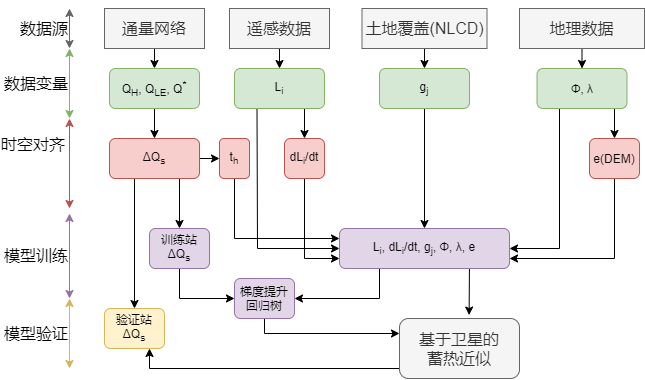
\includegraphics[width=\linewidth]{img/图1.png}
    \end{center}
    \caption{数据源、派生变量,以及模型构建与验证处理的原理图}
\end{figure}

\subsection{剩余蓄热}

在能量平衡闭合假设下,地表能量收支可用于求解热源和热汇之间的蓄热剩余(Oke, 1988; Piringer et al., 2002; Sun et al., 2013; Sun et al., 2017b):

\begin{equation}
    \Delta Q_s=Q^*-(Q_H+Q_{LE})
\end{equation}

其中$\Delta Q_s$表示蓄热通量,$Q^*$是全波长净辐射,$Q_H$和$Q_LE$分别表示显热与潜热通量。通过以上方法得到剩余蓄热是一种直观的方法,并在辐射计和涡度协方差仪器可测量残余通量的情况下常常被使用(Ferreira et al., 2013; Roberts et al., 2020)。假设与$Q_F$有关的误差大于它对能量收支的贡献(Parlow et al., 2014; Sun et al., 2017a),或是涡度协方差仪器被认为能捕捉到大多数人为活动释放的绝大部分辐射、传导或对流(Grimmond and Oke, 2002)时,人为热通量($Q_F$)通常被忽略。

显热和潜热由装有气体分析仪和三维超声波风速计的闭合涡度协方差系统观测得到(Balogun et al., 2009)。净辐射由净辐射计测量得到,它将入射和出射的短波、长波辐射进行平衡(Ando and Ueyama, 2017)。使用了纽约州中尺度网和美国国家生态观测网(NEON)2个网络;因此,在所有站点中可以找到不同的仪器型号。

每半小时获取一次通量数据,以与每个对应的卫星像素进行比较。卫星数据与通量测量的时间对齐到2.5分钟以内(因为卫星观测间隔是5分钟)。无论天气影响如何,16个波段的卫星像素都是可用的,而通量站会自动去除极端风雨天气下的数据。

\subsection{梯度提升回归树(GBRT)}

选择梯度提升回归树(GBRTs)是基于它在多变量系统中的表现及它们不会非线性过拟合的能力(Kedem et al., 2012)。这里使用的GBRT算法类似(Ke et al., 2017)开发的方法,其中变量和观测值之间的差异被计算为“损失函数”并拆分成几部分(称为树)。树的数量由后续添加树在精度上的提升决定。例如,若树的数量增加使误差下降了一定的量,则再添加一棵树,并继续进行划分。若精度逐渐趋近某一个值,则停止添加树(Friedman, 2001; Mason et al., 2000)。这里GBRTs的精度用最小二乘法计算。在梯度提升方面,计算伪残差作为损失函数的梯度,并在每个时间步长中使用,以提高模型的预测能力(Friedman, 2002)。

使用GBRTs、16个卫星辐亮度、16个卫星辐亮度的时间导数,以及地表覆盖和特定的地球物理属性来和剩余蓄热一同训练,正如方程(2)所述。目标是创造一个使用卫星传送的辐亮度数据和地表覆盖及其他现象贡献的健壮的算法。通过使用特定的地表覆盖参数,滞后模型将揭露卫星数据与地面属性之间的潜在关系,使得该算法在未校正地区的使用更加容易。GBRTs对过拟合很敏感,因此将使用独立的站点来评价模型的实际表现。将通过改变训练集大小来探究模型的时间序列依赖,并评价模型的最佳表现(Robinzonov et al., 2012; Schonlau, 2005)。

使用Python的Scikit-learn库(Pedregosa et al., 2011)来实现上述的梯度提升回归树方法(Prettenhofer and Louppe, 2014)。在训练和验证阶段,2019年夏天的剩余蓄热通量将按时间与34个通量站来划分。站点被分为训练组和验证组,还有一些站点单独用于模型的独立验证。数据按时间划分,每个站的数据点按总数百分比输入到GBRT算法中。例如,若一个站有1000个有效数据点,大小为80\%的训练集将使用800个数据点来训练,200个数据点来验证。训练阶段将按序列划分,来优化现实世界情况下的算法。使用序列划分可以使数据以类似的方法在发布产品中使用,其中训练可以在按时更新的数据中连续进行。这使得实时校正和长期的模型整体精度改善成为可能,训练时站点是随机打乱的,意味着不同的训练阶段误差可能变化。这有助于用不同的输入来使模型多样化、测试稳定性,并克服模型可能存在的过拟合缺陷。

\subsection{降尺度步骤}

我们提出了一个简单的、不需要高级工具或机器学习算法训练的降尺度步骤。降尺度可用的参数有NLCD、地理属性、卫星辐亮度,使用更高的空间分辨率参数来创造更高空间分辨率的蓄热地图。该方法输入$2km$的原生算法(它是16个波段中主要的12个的分辨率)并生成$320m$的产品。

NLCD和数字高程模型都有高达$30m$的空间分辨率。因此,假设降尺度程序的功能是准确和线性的,没有引入较大误差,则$30m$分辨率决定了算法可能的最小分辨率。这里提出的降尺度使用了和和气象学有关的不同卫星算法相似的方法(Busch et al., 2012; Mascaro et al., 2010; Ranney et al., 2015)。降尺度卫星产品使用的算法有三种:卫星对卫星方法,使用地理信息数据的方法,以及基于模型的模型(Mitraka et al., 2015; Peng et al., 2017)。合理降尺度卫星数据有关文献中可以找到其中一种方法或几种方法的组合。

这里提到的降尺度取决于蓄热很大程度上依赖土地覆盖比例的假设,意味着机器学习模型对于更高分辨率输入的精确度不会改变。而且由于没有更高空间分辨率和相似的时间或光谱分辨率卫星可比,卫星对卫星方法无法使用。当然,更高分辨率卫星在特定的过境时间内是可用的,而且可能是最好的降尺度方法。然而,由于此处使用的模型是多光谱方法,卫星间进行比较之前需要在光谱上降尺度,这超出了本文范围。由于缺乏高分辨率的地面网络来训练模型,也没有用于与数值模型比较的标准,基于模型的模型方法在本研究中也难以实施。就结果而言,将采用地理信息数据方法来对模型降尺度。

与通量塔比较时这些地理统计假设可能被打破,因为这些文献(Bergeron and Strachan, 2011; Feigenwinter et al., 2017; Kotthaus and Grimmond, 2012; Kotthaus and Grimmond, 2014; Velasco et al., 2005; Velasco et al., 2009)提到通量塔在城市区域的测量范围是$0.5km\sim2km$。然而,这将在后面结果展示的章节中进行评估。

\subsection{误差度量}

即将进行分析的滞后模型使用标准的统计方法将地面站剩余通量数据与它的表现进行比较。以下是比较模型蓄热通量和真实站点蓄热通量间残差的相关指标(Şahin, 2012; Laurent et al., 1998; Singh and Irmak, 2009)

\begin{equation}
    RMSE=\sqrt{\frac{1}{N}\sum_{i=1}^N(\Delta Q_{s,i,model}-\Delta Q_{s,i,station})^2}
\end{equation}

\begin{equation}
    MAE=\frac{1}{N}\sum_{i=1}^N|\Delta Q_{s,i,model}-\Delta Q_{s,i,station}|
\end{equation}

\begin{equation}
    MBE=\frac{1}{N}\sum_{i=1}^N(\Delta Q_{s,i,model}-\Delta Q_{s,i,station})
\end{equation}

\begin{equation}
    R^2=1-\frac{\sum_i(\Delta Q_{s,i,model}-\Delta Q_{s,i,station})^2}{\sum_i(\Delta Q_{s,i,station}-\overline{\Delta Q_{station}})^2}
\end{equation}

其中$RMSE$代表均方根误差(root-mean-square error),$MAE$是平均绝对误差(mean-absolute error),$MBE$是平均偏差误差(mean bias error),$R^2$是决定系数(coefficient of determination),有时称作模型效率。这四个指标可以归一化本文中的比较,本文使用了其中的若干种指标。

\section{地理环境与数据选择}

\subsection{研究区域}

研究区域包括了$16\times24$个$2km$尺度的GOES-16卫星像元格网。使得原生的基于卫星算法在纽约市地区有共计384个像元。总共34个站点被用于分析,其中20个来自NEON,10个来自Ameriflux,3个来自NYS Mesonet,1个来自纽约市立大学城市学院。观测时间为2019年6月至8月,观测站的地理分布仅限于美国大陆(continental United States, CONUS)中。所有站点都使用不同比例的可用数据进行了训练,但特定的城市分析仅限于纽约市内的4个城市站点。图2展示了4个纽约市的通量站在NLCD纽约市地图上的分布。从图2可见,研究区域以开放水域和建成区土地覆盖为主。

\begin{figure}[htbp]
    \begin{center}
        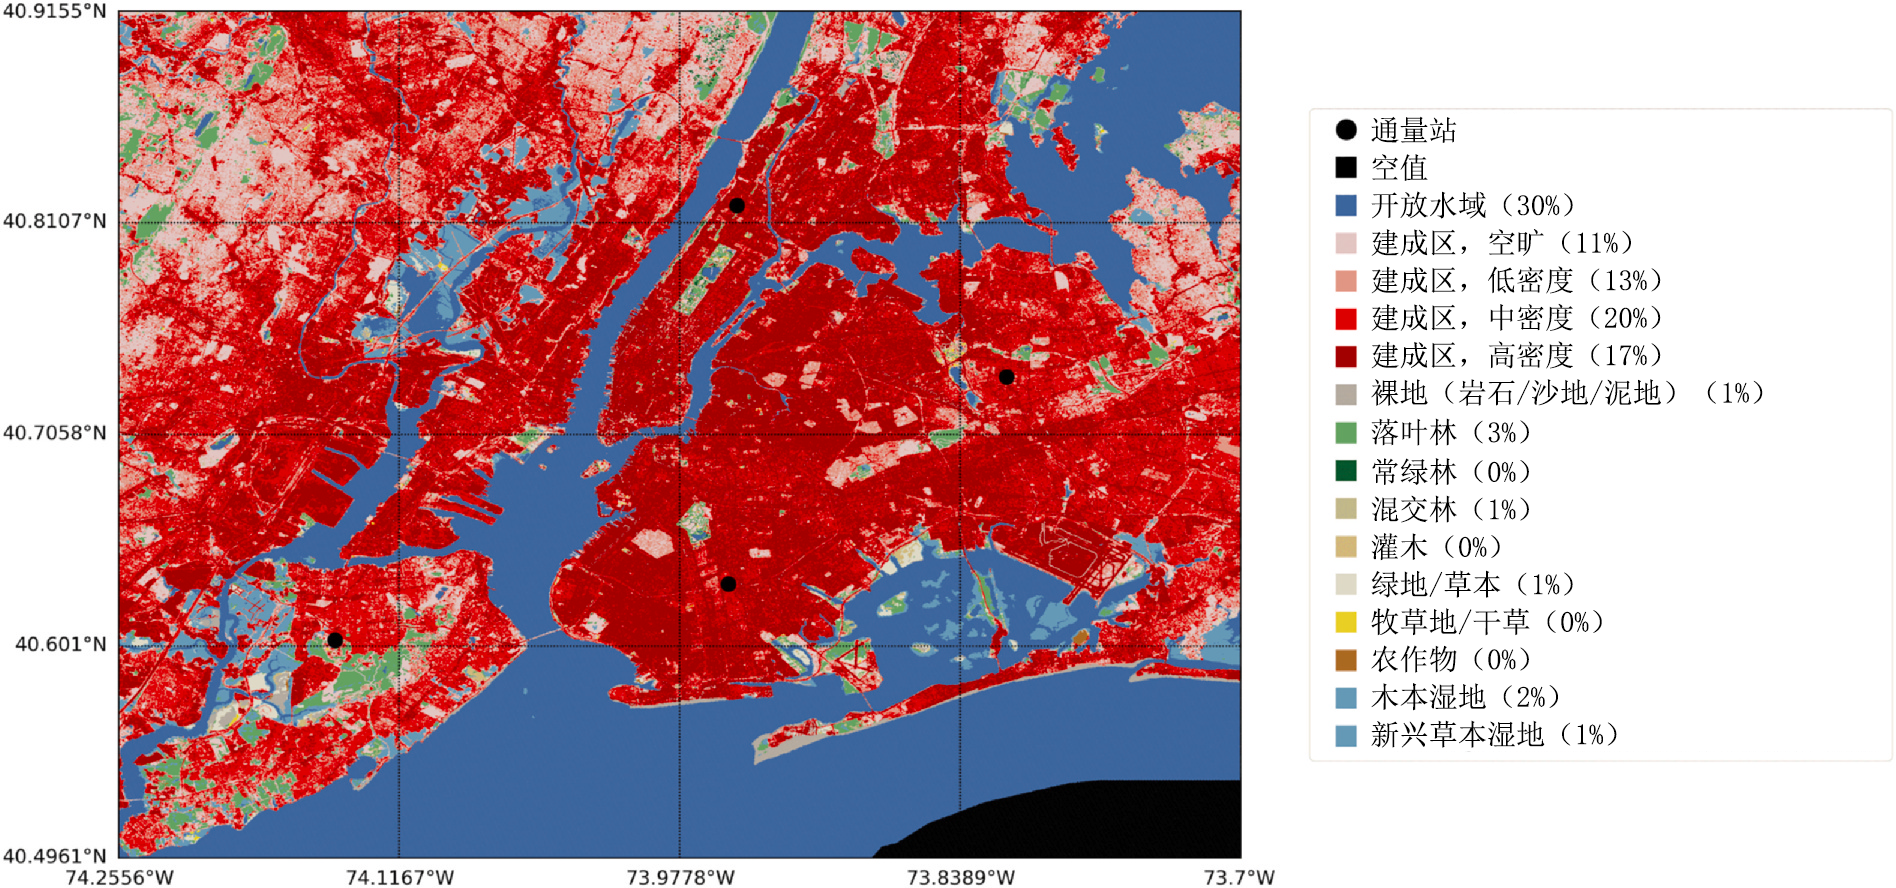
\includegraphics[width=\linewidth]{img/图2.png}
    \end{center}
    \caption{通量站分布和NLCD纽约市土地覆盖地图}
\end{figure}

\subsection{地表通量站点}

3个网络被用于分析:美国国家生态观测网(the National Ecological Observatory Network, NEON)、美洲通量网(the Ameriflux network),以及纽约州中尺度网(the New York State Mesonet)。每种网络的通量都由涡度协方差方法(Network, 2020a)得到。NEON站点使用安装在垂直塔顶的Campbell Scientific CSAT-3声波风速仪和Li-Cor LI-7200气体分析仪。使用原始数据生成显热和潜热通量的30分钟湍流通量数据产品。净辐射由Hukseflux NR01净辐射计获取的入射和出射短波和长波辐射成分得到。共计21个NEON站点中的大多数位于非城市区域,有助于分开NYS Mesonet城市站点的土地覆盖植被成分。

Ameriflux核心站点与NEON站点一同使用,并且采用了和Campbell Scientific and Li-Cor相似的通量塔和气体分析仪(Ameriflux, 2020)。使用了Ameriflux网络中的9个站点,其中的大部分都位于非城市区域。Ameriflux站点的引入增加了卫星算法训练及验证的多样性。与NEON网络相似,显热和潜热通量及净辐射每30分钟获取一次并生成蓄热剩余。

最后的地面网络是NYS Mesonet。NYS Mesonet站点使用Kipp \& Zonen CNR4净辐射计、Campbell Scientific CSAT3A 3D超声波风速计和EC155气体分析仪。NYS Mesonet站点的仪器也每30分钟记录一次显热、潜热和4成分的辐射。特别使用了3个城市区域的NYS Mesonet站点,且都位于纽约市。还有一个通量塔位于曼哈顿的纽约市立大学城市学院,它与NYS Mesonet的仪器是一样的,但不由NYS Mesonet维护。最后共计34个地面通量站用于分析。城市站点是卫星步骤最好的测试平台,也将成为机器学习步骤的性能基准。

\subsection{GOES-16卫星数据}

地球同步运行环境卫星-R系列(The Geostationary Operational Environmental Satellite-R Series, GOES-R)在到达其运行轨道后更名为GOES-16。将它被用作气象卫星来和从通量网络NEON和NYS Mesonet获取的地基剩余蓄热通量进行比较。原始的光谱辐亮度数据通过先进的基线成像仪(the Advanced Baseline Imager, ABI)以称为L1b(Level 1b)的数据格式获取,它在谷歌大查询数据库(Google BigQuery database)上对所有人开放获取。

L1b光谱辐亮度使用的单位是$[W\cdot m^{-2}{sr}^{-1}{\mu m}^{-1}]$。使用的GOES-16扫描模式3每5分钟观测一次美国大陆(CONUS),得到16个波段。这使得地基的通量站和对应的卫星像元的时间对齐精度达到了2.5分钟。相邻像元的空间分辨率取决于所选波段,大致上从$0.5km$到$2km$(Group, G.C.W, and Program, 2017)。

\subsection{土地覆盖和数字高程模型}

美国地质调查局最近发布了第五版的美国国家土地覆盖数据库(National Land Cover Database, NLCD),命名为NLCD2016。这里使用的是美国大陆(CONUS)NLCD2016产品,它被处理为了$30m$空间分辨率和16种土地覆盖类型的产品(Jin et al., 2019; Wickham et al., 2014; Yang et al., 2018a)。类型被分为了以下几种:开放水域;多年冰/雪;空旷的、低密度的、中密度的和高密度的建成区;裸地(岩石/沙地/泥地);落叶的、常绿的、混交的森林;灌木;绿地/草本;牧草地/干草;农作物;木本的、新兴草本的湿地。纽约市的NLCD划分见图2。NLCD2016包含了4种城市类型(建成区类型)且将决定给定卫星像元的城市化程度。

与16个NLCD类型一起,一种数字高程模型(digital elevation model, DEM)将成为每个卫星像元分类的一部分。航天飞机雷达地形测绘任务(the Shuttle Radar Topography Mission, SRTM)由美国地质调查局推动,发布了一个自由获取的、$30m$分辨率覆盖整个美国大陆的高程产品(Elkhrachy, 2018)。给定卫星像元的经纬度坐标决定了高程,并用于机器学习算法来捕捉蓄热对高程和土地类型变化的敏感性。这在基于卫星的地表蒸散或热力学过程评估中很常见(Cheng et al., 2011; Semmens et al., 2016; Xian and Crane, 2006; Zhou et al., 2014)。DEM和NLCD的分辨率都远高于卫星,有助于最终卫星算法的降尺度。

\subsection{卫星波段和剩余蓄热的关系}

研究的假设取决于卫星辐亮度和地面站剩余蓄热间的相关性。若如这些文献(Bisht and Bras, 2010; Carmona et al., 2015; Hou et al., 2014; Jin et al., 2011)通过卫星辐亮度得到了净辐射,不含预测净辐射这一中间步骤的原始辐亮度的应用也许足以直接近似蓄热。特别的,由于16个高时间分辨率的波段覆盖了可见光、近红外和红外波长(Schmit et al., 2018),卫星辐亮度和蓄热间的相关性应当很高。图3显示了一个城市区域(纽约的布鲁克林)地面站和最近的卫星像元间的相关性,其中变量间的相关性定义为(Benesty et al., 2009; Inglada, 2002):

\begin{equation}
    Corr=\frac{\sum_{k=1}^N(\Delta Q_{s,k}-\overline{\Delta Q_s})\cdot(L_{\lambda,k}-\overline{L_\lambda})}{\sqrt{\sum_{k=1}^N(\Delta Q_{s,k}-\overline{\Delta Q_s})^2}\cdot\sqrt{\sum_{k=1}^N(L_{\lambda,k}-\overline{L_\lambda})^2}}
\end{equation}

\begin{figure}[htbp]
    \begin{center}
        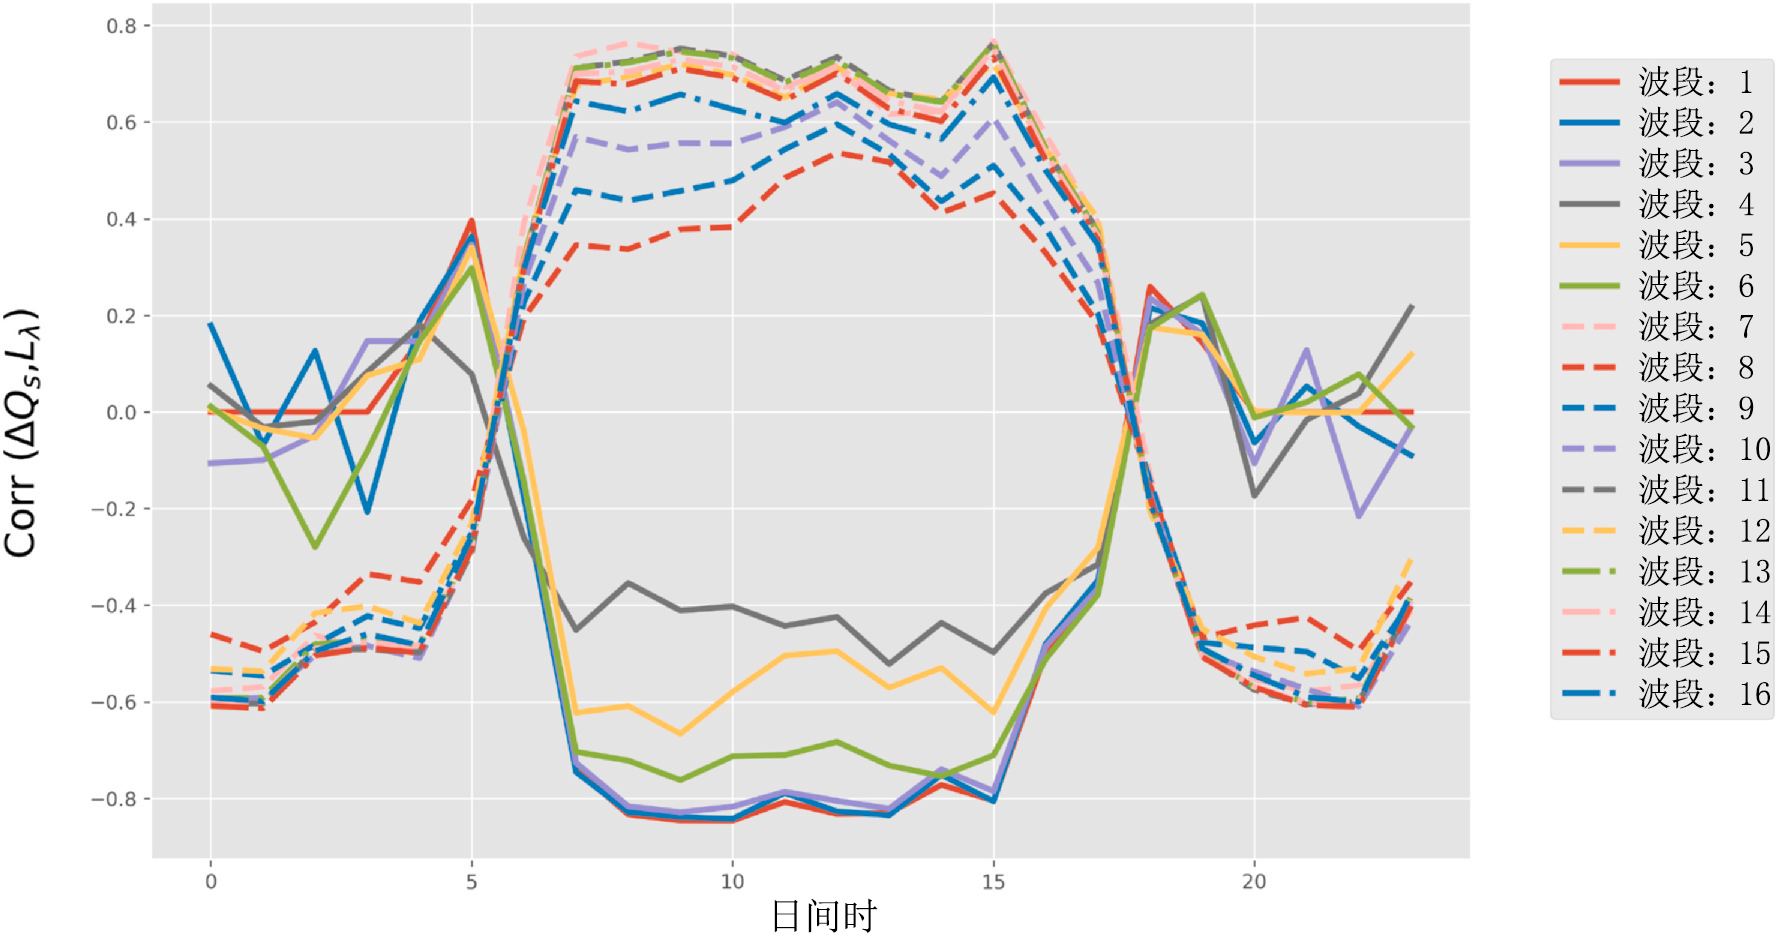
\includegraphics[width=\linewidth]{img/图3.png}
    \end{center}
    \caption{地面站剩余蓄热通量与最近的GOES-16所有波段像元间的相关性。短波波段在白天与蓄热通量负相关,在夜间的相关性很小;而长波波段在白天与蓄热通量正相关、在夜间呈负相关。这些相关关系对辐亮度波段可用于计算蓄热通量的假设至关重要。}
\end{figure}

短波波段在白天可视为与蓄热通量呈负相关,应该是受太阳直接辐照的影响。在夜间短波波段和蓄热几乎没有相关性,正如与之前相反的原因所预期的那样。对于长波波段,在夜间和白天都有很高的相关性。长波波段在白天与蓄热通量正相关,在夜间则呈负相关。这些相关关系巩固了最初GOES-16辐射波段能用于计算蓄热通量的假设,这个假设也是本研究的主要动力所在。

\section{结果与讨论}

\subsection{训练与验证}

由于当地气象条件的变化性(狂风、暴雨)和设备的复杂性两种数据劣化的原因,训练和验证在可用站点的范围内都不是统一的。这在整个测试阶段每个站点的数据数量都是不同的。图4显示了训练阶段和验证阶段的平均RMSE,其中训练数据集是由来自所有3个网络的21个地面站组成的独特集合,而独立数据集是所有3个网络中剩下的13个地面站组成的独特集合。

\begin{figure}[htbp]
    \begin{center}
        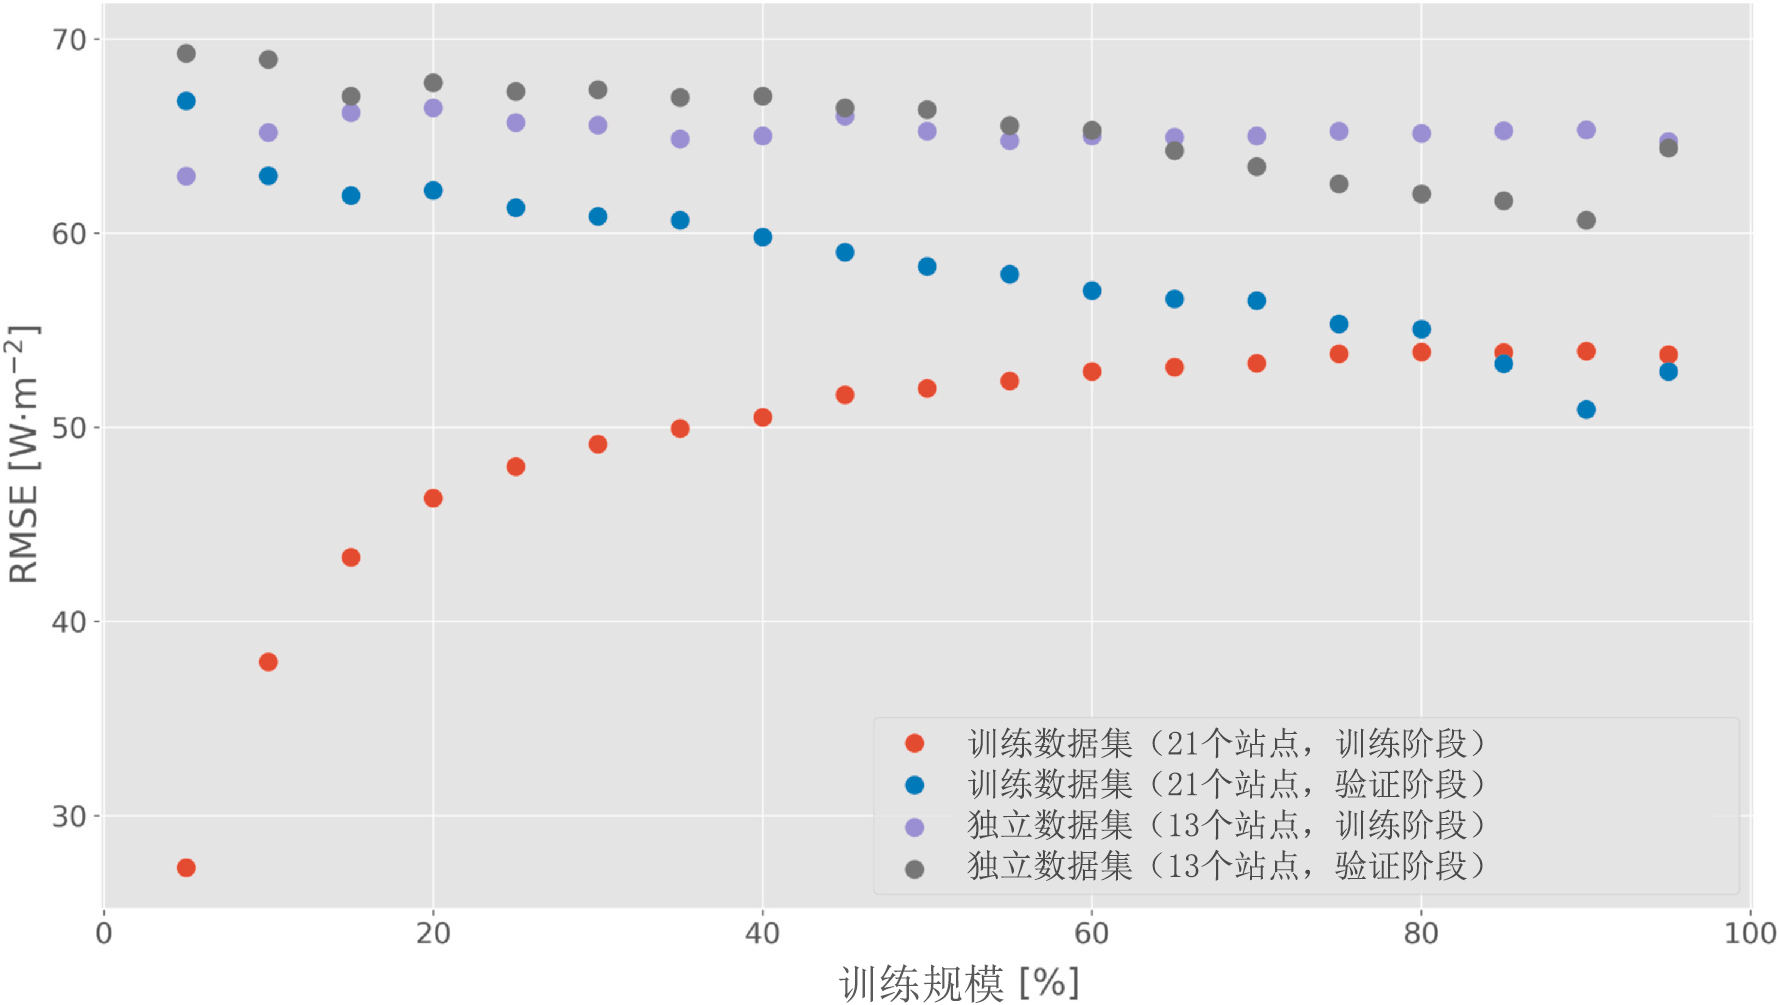
\includegraphics[width=\linewidth]{img/图4.png}
    \end{center}
    \caption{RMSE是训练数据集和独立数据集中训练规模的函数。训练数据集和独立数据集都被分为了训练阶段和验证阶段。可见在验证阶段RMSE如预期般随着训练规模的增加而降低}
\end{figure}

图4给出的曲线随着训练规模的变化呈现预期的行为。训练数据集在整个训练阶段的误差都是最低的,原因很可能是过拟合——一种GBRT算法中的常见缺陷(Kedem et al., 2012)。同样的,验证阶段的误差也低于独立数据集。然而,独立数据集在整个训练规模范围内都表现出连贯的误差,表明训练与训练规模间有一定的稳定性,误差随着训练规模的增加而略有下降。

参考图4的结果,选取90\%的数据来训练,10\%的数据来验证。因为80\%是训练和验证误差趋近的标志,选取任意大于80\%的训练规模都是有效的。独立数据集也经历了相似的现象,而且其变化更小,表明模型与独立地面站点(或卫星像元)有关的真实预测精度更高。

表1给出了与基于卫星的GBRT模型在90\%训练规模时有关的统计。考虑到卫星滞后模型的表现,可以给出一个结论性的参数,即与基于地面的剩余热通量相比,$2km$空间模型伴随着$50\sim65 W\cdot m^{-2}$的误差。当然,这只是针对2019年的夏天。这个论断的有效性仍需在多个季节进行进一步的验证。

\begin{table}[htbp]
    \caption{2019年夏天的训练和验证数据划分分析}
    \centering
    \begin{tabular}{ccccc}\hline
        数据集&阶段&\# 站点数&平均 \# 点数&RMSE\\
        \hline
        训练&训练&21&2927&55.8\\
        训练&验证&21&326&52.6\\
        独立&训练&13&2594&63.7\\
        独立&验证&13&289&60.5\\
        \hline
    \end{tabular}
    
\end{table}

\subsection{纽约市案例研究}

图5给出了纽约市4个城市站点的验证阶段的散点图。其中2个城市站点参与了训练(BKLN和CCNY),而另2个没有(QUEE和STAT)。对于所有4个站点,RMSE值都低于$60W\cdot m^{-2}$,MAE都低于$43W\cdot m^{-2}$。城市区域的RMSE和MAE的平均值分别为$49$和$34W\cdot m^{-2}$。MBE的平均值为$7.6W\cdot m^{-2}$,$R^2$的均值为$0.83$。所有4个表现指标都在文献(Roberts et al., 2006)引用范围之内。

\begin{figure}[htb]
    \begin{center}
        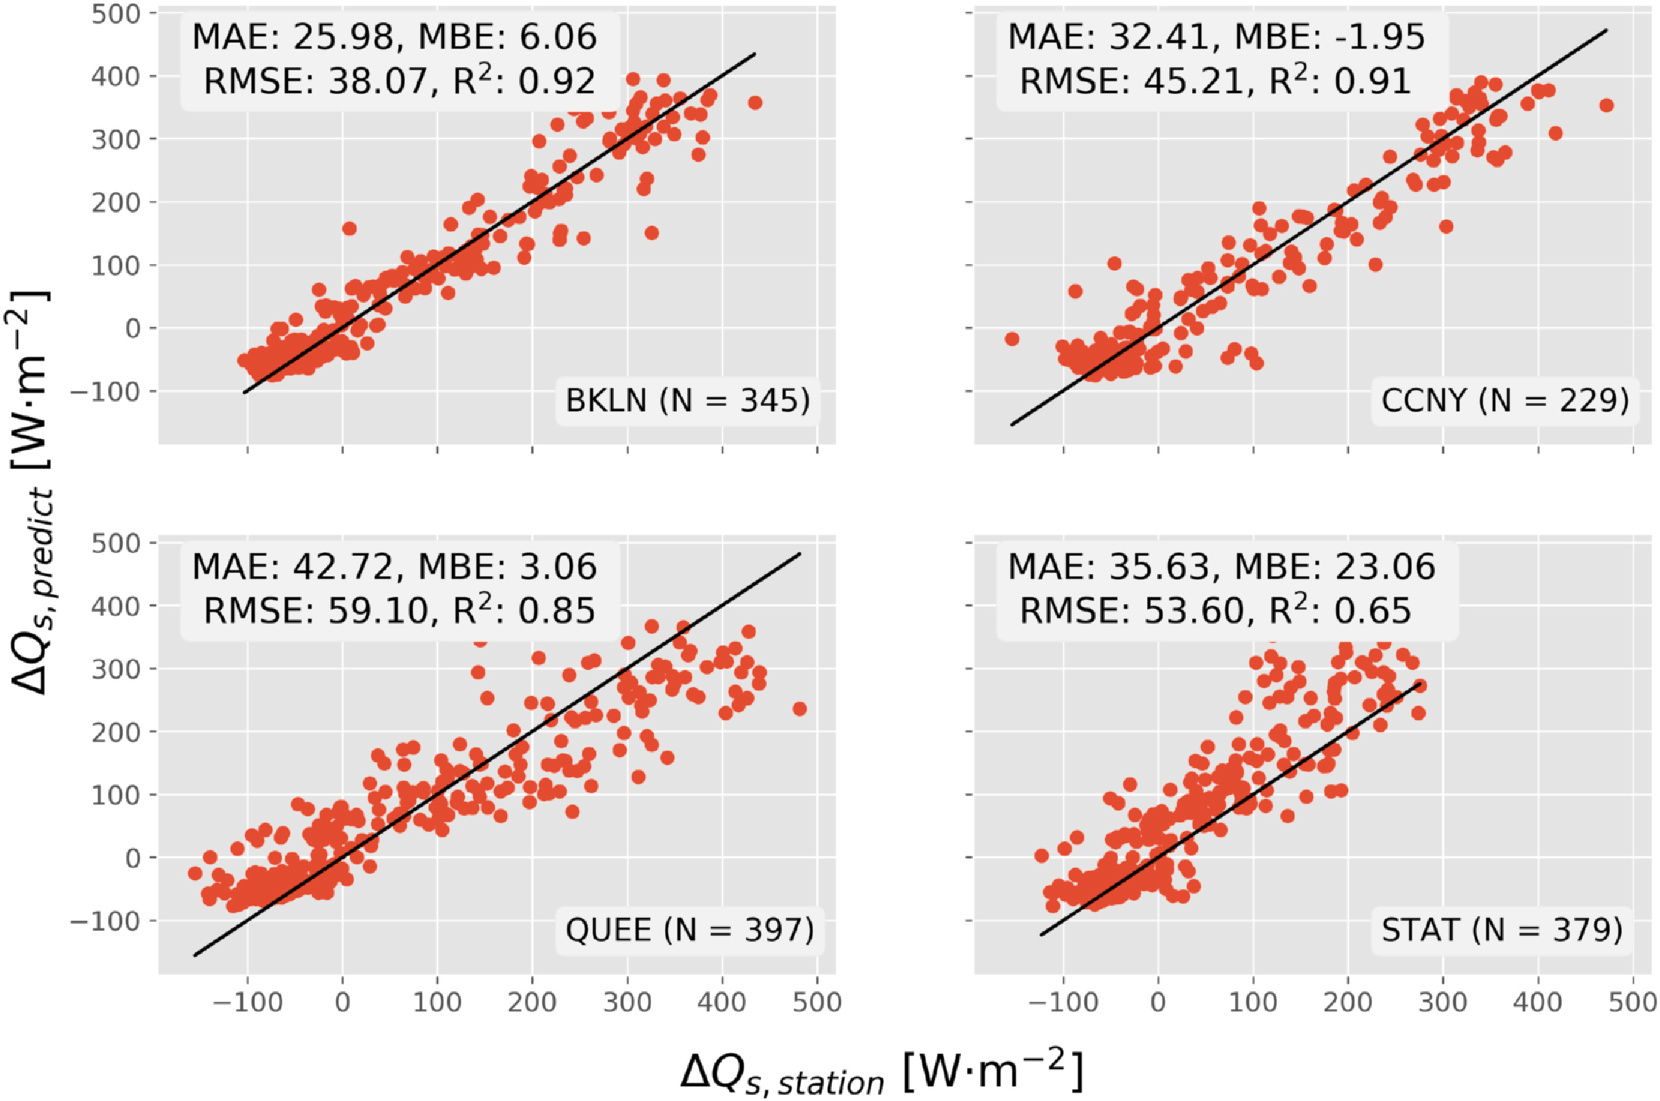
\includegraphics[width=\linewidth]{img/图5.png}
    \end{center}
    \caption{NYC通量站点和使用GOES-16卫星的模型表现}
\end{figure}

图6是对与图5中验证数据同样的集合进行的时间重建。时间重建的阵列能有效追踪$\Delta Q_s$的日间曲线,这是目前卫星研究中没有涉及过的(Chrysoulakis et al., 2018; Kato and Yamaguchi, 2007; Parlow, 2003; Rigo and Parlow, 2007)。卫星滞后模型也能在雨天和多云时估计蓄热,也是这些卫星文献缺乏的能力。在8月22日、23日和28日,纽约市地区的历史天气记录显示是云雨天气,这一点由图6中蓄热更小的振幅体现。

\begin{figure}[htb]
    \begin{center}
        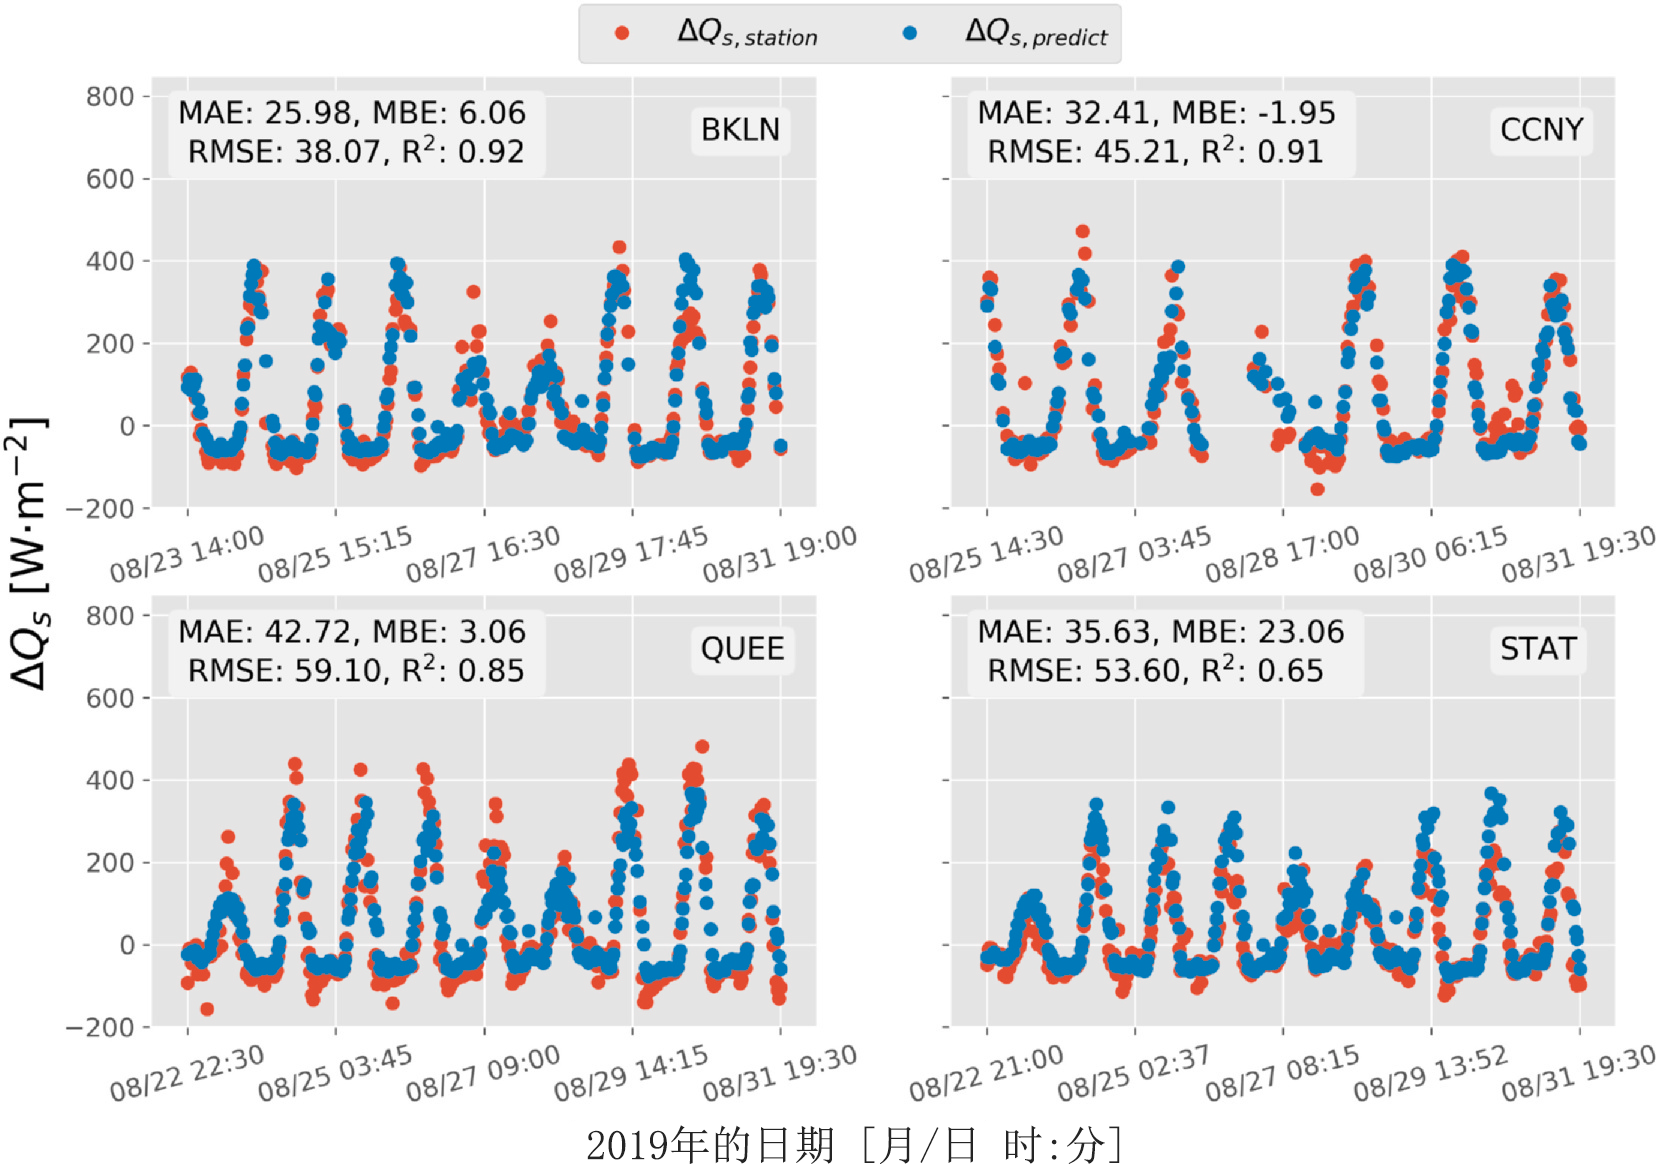
\includegraphics[width=\linewidth]{img/图6.png}
    \end{center}
    \caption{使用卫星滞后模型对$\Delta Q_s$进行时间重建}
\end{figure}

该模型能重现大多数日循环内每个站点的蓄热趋势。该模型最与众不同的一点在于它能捕捉到白天最大值和夜间最小值的完整振幅。对皇后站(Queens, QUEE),能观测到蓄热的白天峰值比站点剩余值更小,夜间则相反。对斯塔滕岛站(Staten Island, STAT),白天峰值不知为何被卫星高估了,也许能归因于统计偏差。

因为训练数据集中没有QUEE和STAT,我们假设基于卫星的$\Delta Q_s$或许在城市区域较少的站点有正偏差(STAT岛只有约60\%属于土地分类中的建成区),并且对城市区域白天和夜间的振幅有更缓和的反应(QUEE的现象,QUEE的土地覆盖类型几乎100\%是建成区)。然而,需要更多的城市站点来充分证实这一主张。

需要注意的是,BKLN和CCNY这2个训练站点都是几乎100\%的城市类型,意味着每个站点和卫星像元对相似的土地覆盖有不同的反应。这是一个重要的现象,它增加了在地面站点不可用于比较的情况下,模型捕捉不同城市环境反应的能力的可信度。尽管QUEE的误差高于其他3个站点,它仍然远小于所有基于地面的OHM方法文献的误差范围,表明卫星步骤在量化蓄热方面是可行的。接下来的几章将继续讨论引入降尺度步骤后的误差。

\subsection{从$2km$降尺度到$320m$}

围绕纽约市陆地块的无处不在的水是开发卫星算法过程中的巨大障碍。这个问题是训练算法时出现的,水体区域没有地面站,这是含有一定水的像元的弱点。结果而言,水体比例大于$0.05(\%5)$的像元被剔除。由于基于卫星的蓄热输出结果原生分辨率为$2km$,研究区域的许多像元都被剔除了。

为了增加纽约市小窗口中卫星像元的数量,使得那么多像元不必因为含水而被剔除,我们开发了一个降尺度步骤。它将卫星算法从$2km$降尺度至$320m$,减少了剔除的像元数,使得蓄热在城市中的分布表现更好。这对于水体高度包围城市区域的沿海城市意义非凡。

正如2.4章解释,基于卫星的蓄热原生分辨率是$2km$,设定源于辐亮度波段的主要空间分辨率。在此设置降尺度到$320m$,将纽约市网格的分辨率增加到了$100\times150$。降尺度算法在QUEE和STAT进行了实施验证,其中QUEE的RMSE降低了$5.4W\cdot m^{-2}$,STAT降低了$0.3W\cdot m^{-2}$。如图7所示。同样的现象也出现在BKLN和CCNY站,在比较$2km$像素与降尺度后的$320m$时,发现误差完全没有超过$2W\cdot m^{-2}$。我们对地面站的邻近像元进行了敏感性分析,在毗邻像元发现了相似的结果。它们由于土地覆盖的变化出现了边际变化。此后使用GBRT方法基于卫星的蓄热获取将基于$320m$,结果经过降尺度展示。

\begin{figure}[htbp]
    \begin{center}
        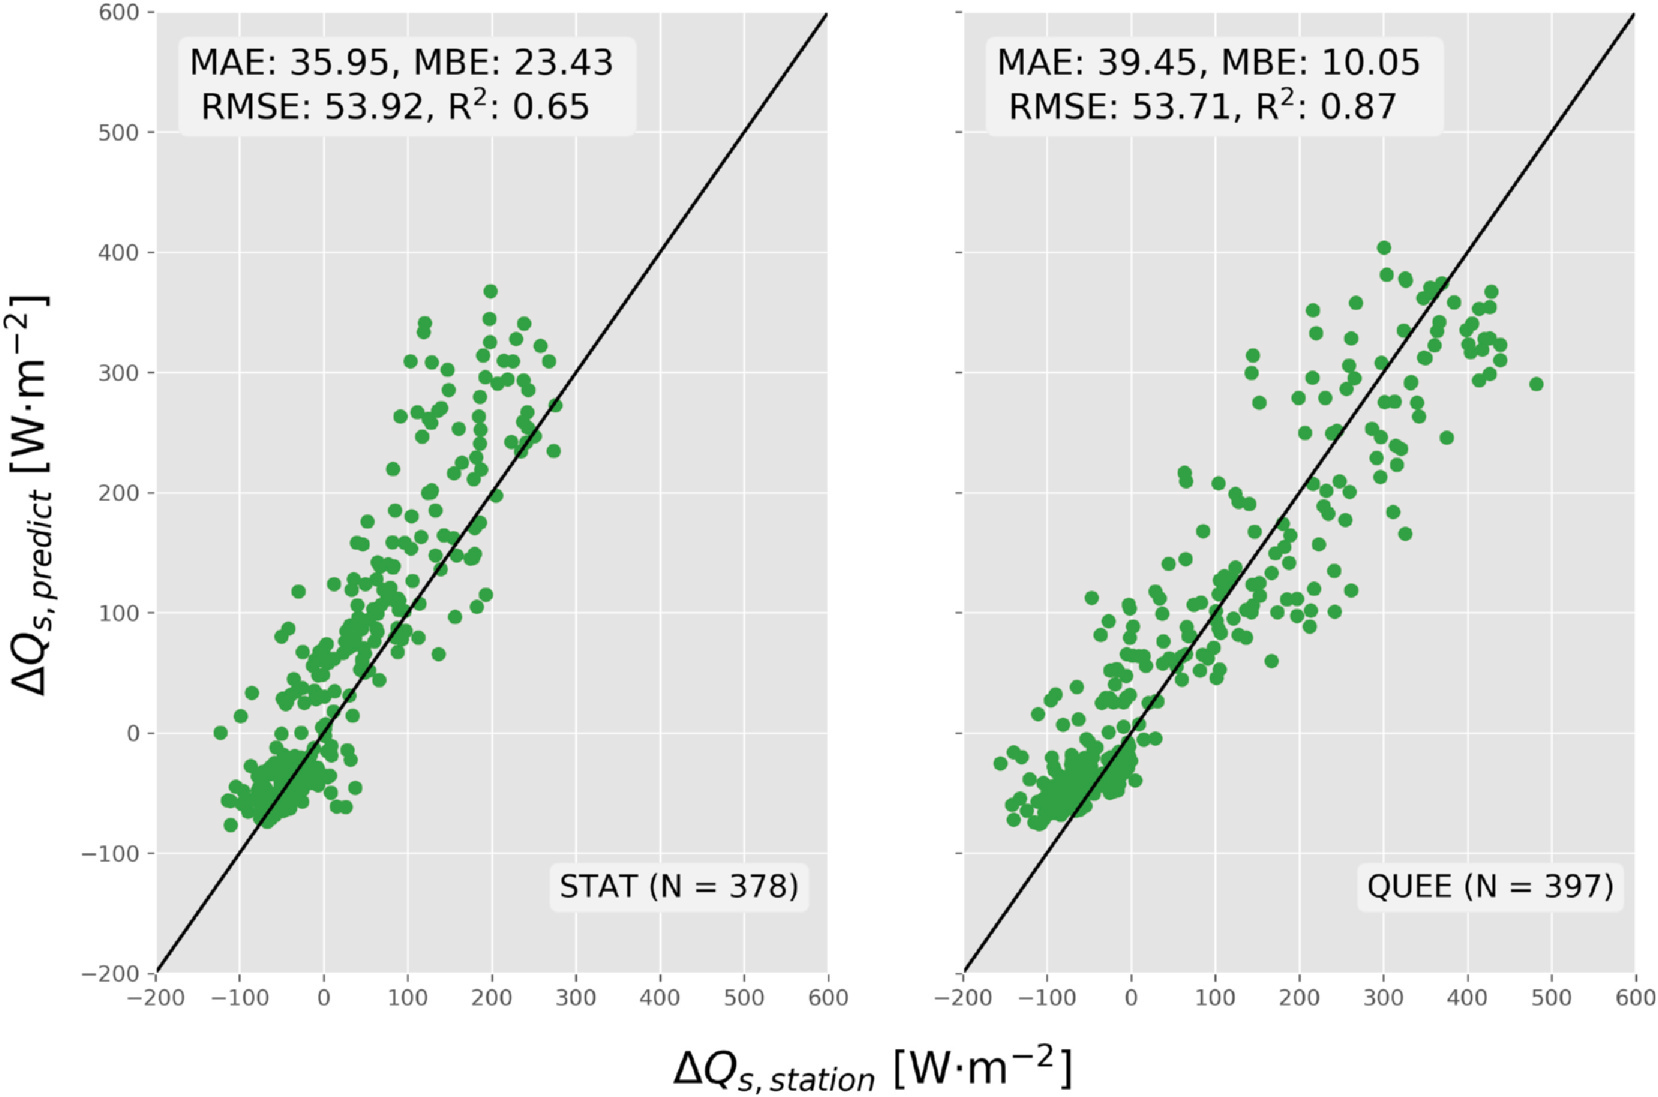
\includegraphics[width=\linewidth]{img/图7.png}
    \end{center}
    \caption{对STAT(左)和QUEE(右)站点进行降尺度的表现。从$2km$降尺度到$320m$使得RMSE在QUEE的像元降低了$5.5W\cdot m^{-2}$,而在STAT像元没有变化,部分验证了降尺度程序的准确性}
\end{figure}

\subsection{蓄热的空间表现}

图8显示了2019年8月24日正午和午夜时期使用卫星滞后模型的蓄热空间表现。数据已如前一章节所述按常规步骤降尺度,结果的分辨率为$320m$而不是$2km$。对水体进行了空间域滤波,水体比例大于$5\%$的像元都被舍弃。另外,基于若干标准差平均最大最小值的观测,任何超出$[-200, 600]W\cdot m^{-2}$的像元也被舍弃。

\begin{figure}[htbp]
    \begin{center}
        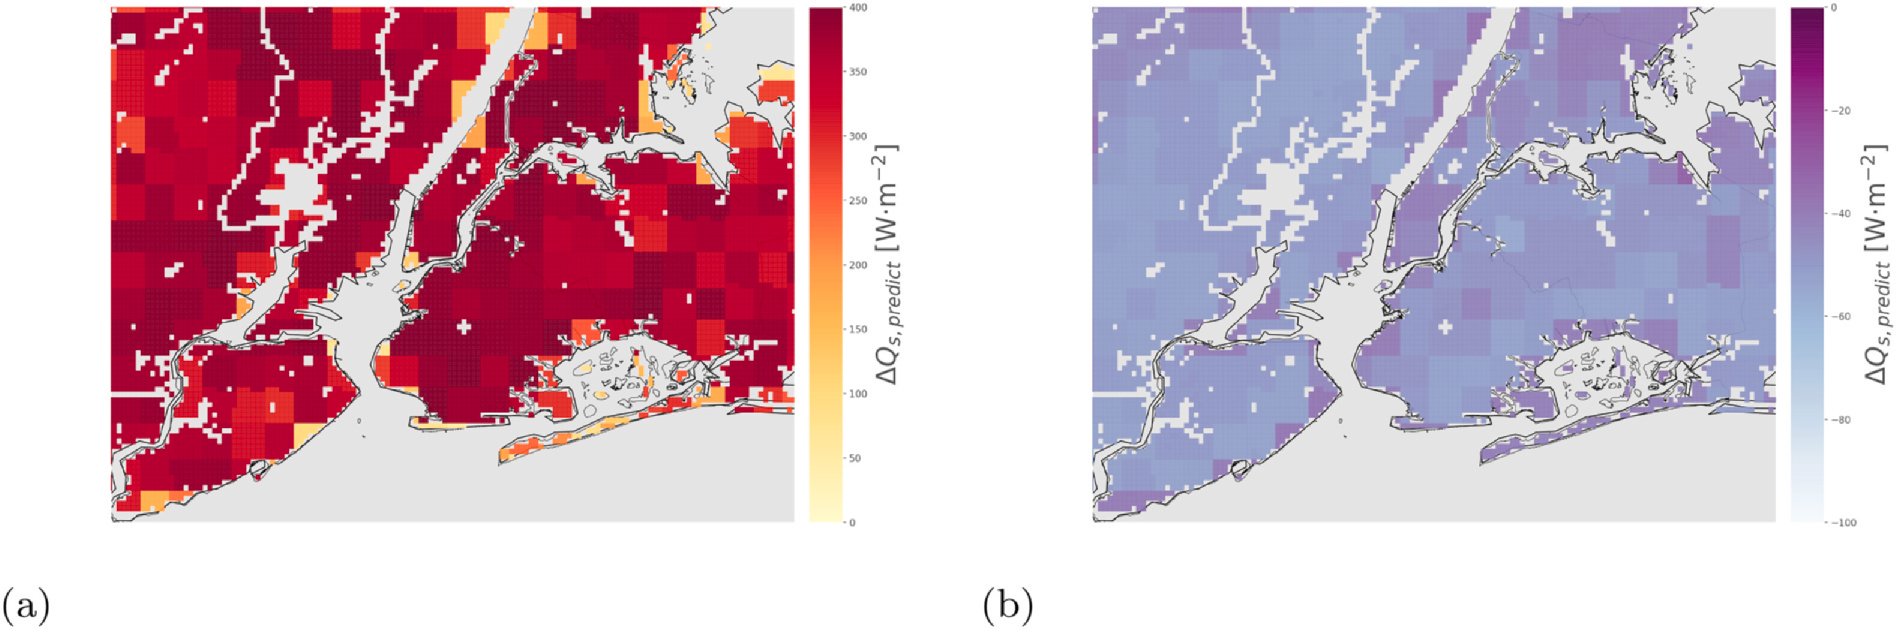
\includegraphics[width=\linewidth]{img/图8.png}
    \end{center}
    \caption{(a)白天的蓄热代表,8月24日EDT时间12:00的$\Delta Q_s$。(b)夜间蓄热的代表,8月24日EDT时间1:30的蓄热。}
\end{figure}

第一个也是最明显的推论是原生$2km$的像元对每个降尺度像元起主要影响。空间域的颜色分布似乎被每个潜在的$2km$像元主导,在图8中的2幅图中都有方形的假象。这可能是由于GBRT模型中的变量优先级,即时间和辐亮度波段优先于土地覆盖和高程。简单地说,这表明模型对于地理的宏观变化更加敏感,而不是地里的局部变化。这也需要归因于卫星的观测角度或高程的巨大变化。

正负通量的转变在蓄热的空间表现中可见。例如,图9a捕捉到了8月27日的日出,整个城市的蓄热变化很大。观测到那天的日出是在早上6:18,表明某些地区的蓄热可能会有延迟效应。图9b也显示了同样的情况,在加热峰值后几个小时的下午5:30,热释放(负蓄热)可见于若干像元,其他则为正蓄热。这是另一项可能的空间延迟。

\begin{figure}[htbp]
    \begin{center}
        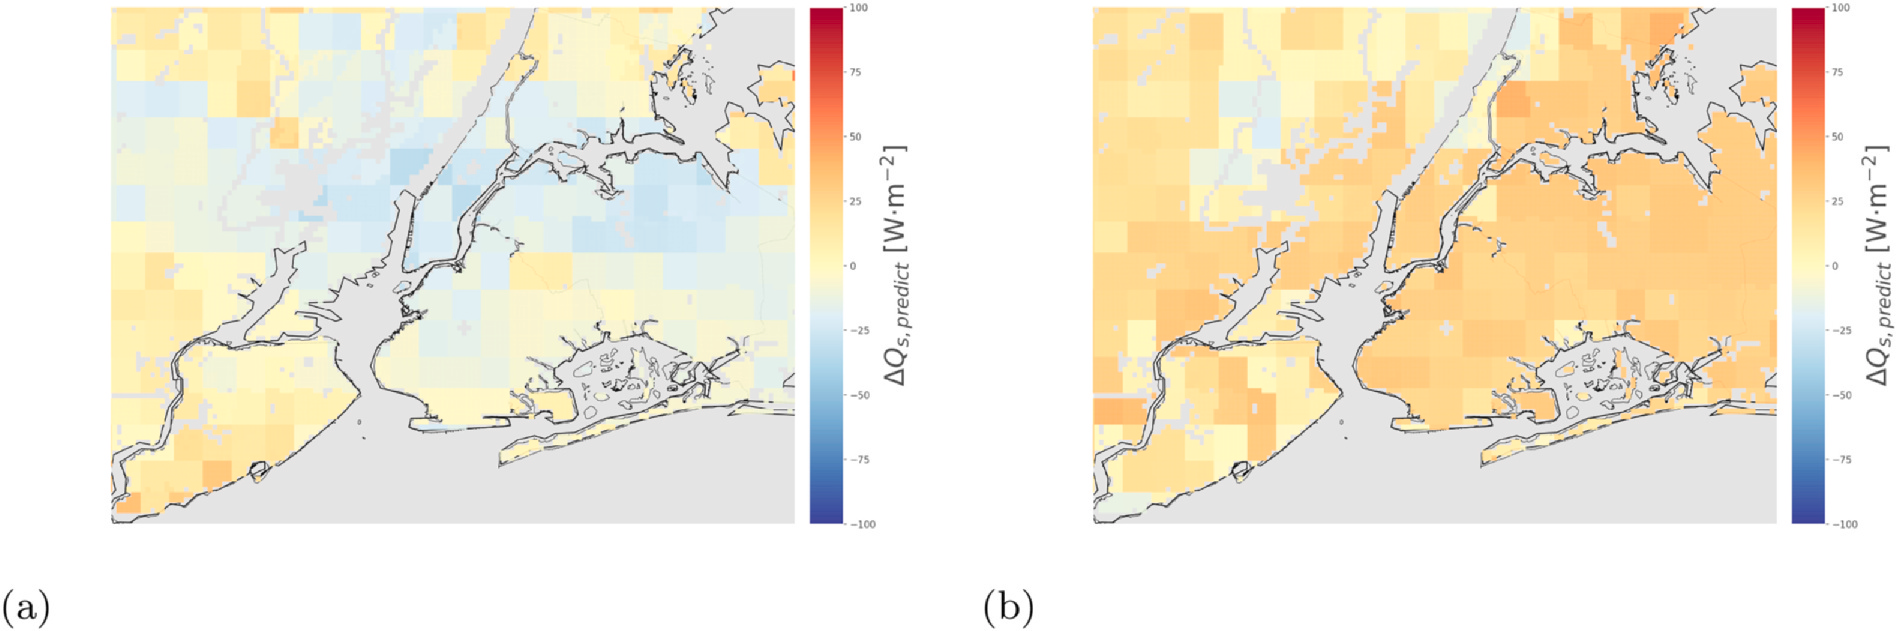
\includegraphics[width=\linewidth]{img/图9.png}
    \end{center}
    \caption{(a)日出之后(8月27日EDT时间7:30)蓄热捕捉到的城市对地表加热响应变化(b)8月27日EDT时间18:30日落后不久,蓄热开始逆转(过零点)}
\end{figure}

全天都可观测到$\Delta Q_s$在各有效像素中标准差的变化。正午的蓄热空间分布变化高达$\pm65W\cdot m^{-2}$,夜间则低至$\pm W\cdot m^{-2}$(原文如此)。这些值相对$\Delta Q_s$的平均振幅为$15\sim20\%$。最大变化发生在图9中的转变时期,在加热峰值几个小时后的日落。

\subsection{与文献的对比}

由于没有可识别的文献将其模型与地面站数值验证,基于卫星的蓄热算法间的统计比较几乎无法实现。因此,无法比较卫星对卫星的表现。这可能是由于缺乏蓄热的测量标准,也可能由地面站在城市的分布稀疏导致。文献也有调查蓄热占净辐射的比例。这在我们的案例中也是不可能的,因为净辐射是剩余方法的一部分,并被用于训练模型。

基于GBRT的方法有一个明确的优势,它避免了作用于城市区域的卫星算法的一个常见缺陷,即对非朗伯表面的处理。这可能要归功于多光谱数据的纳入,它可以处理反射辐射中的一些城市异质性问题(de Almeida Castanho et al., 2007; Hamedianfar and Shafri, 2015)。此外,卫星的时间分辨率也使得大规模的模型与地面站统计比较成为可能,这对算法的单值性和稳定性有所帮助。例如,MODIS日循环内的比较仅限于每天2个比较点。

对卫星滞后模型更合适的评价是通过与基于地对地测量的计算统计进行比较。如简介部分提到的,相关文献中有4种计算蓄热的方法:剩余法(RES),目标滞后模型(OHM),热质法(TMS),小镇能量平衡(TEB)。(Roberts et al., 2006)这篇广受认可的文献进行了一次所有4种方法的比较,并包括对OHM, TMS, TEB相对于RES方法的误差分析。它还汇集了其他研究来努力证实其统计结果。这些误差在这里将指导并部分验证卫星滞后模型的处理结果。

表2展示了滞后模型计算14种不同的蓄热间的比较,其中4种包括纽约市基于卫星的结果。总体而言,皇后(Queens, QUEE)、布鲁克林(Brooklyn, BKLN)、曼哈顿(Manhattan, CCNY)和斯塔滕岛(Staten Island, STAT)这些纽约站在均方根误差上都优于10个站点中的7个。这很了不起,特别对独立验证的STAT和QUEE站而言。所有4个纽约市站点的验证数据点都多于10个站点中的6个。这些统计表明基于卫星的蓄热模型相对地基的OHM方法更加可行。

\begin{table}[htb]
    \centering
    \caption{基于卫星的滞后模型与目标滞后模型方法在多个城市地表净辐射数据的对比。加粗部分为本实验降尺度与最近NYC地面站比较的结果。表格按RMSE升序排列。}
    \begin{threeparttable}
    \begin{tabular}{llll}\hline
    站点/描述&\# 点数&$R^2$&RMSE\\\hline 
    洛杉矶,加利福尼亚 (郊区)\tnote{a}&424&0.92&29.0\\
    墨西哥城 (城市中心)\tnote{a}&61&0.96&33.6\\
    \textbf{布鲁克林,纽约(城市)}&\textbf{345}&\textbf{0.92}&\textbf{39.5}\\
    \textbf{曼哈顿,纽约(城市)}&\textbf{229}&\textbf{0.91}&\textbf{45.0}\\
    温哥华,加拿大(工业)\tnote{a}&312&0.88&48.9\\
    \textbf{皇后,纽约(城市)}&\textbf{397}&\textbf{0.87}&\textbf{53.7}\\
    \textbf{斯塔滕岛,纽约(郊区)}&\textbf{379}&\textbf{0.65}&\textbf{53.9}\\
    迈阿密,佛罗里达(郊区)\tnote{a}&204&0.79&61.9\\
    温哥华,加拿大(郊区)\tnote{a}&464&0.67&62.9\\
    萨克拉门托,加利福尼亚(郊区)\tnote{a}&222&0.56&66.0\\
    圣保罗,巴西(郊区)\tnote{a}&353&0.69&74.1\\
    芝加哥,伊利诺伊(郊区)\tnote{a}&163&0.56&83.3\\
    马赛,法国(城市中心)\tnote{b}&192&0.70&94.8\\
    图森,亚利桑那(郊区)\tnote{a}&75&0.75&107.4\\\hline
    \end{tabular}
    \begin{tablenotes}
        \item[a] Grimmond and Oke (1999)
        \item[b] Roberts et al. (2006)
    \end{tablenotes}
    \end{threeparttable}
\end{table}

至于小镇能量平衡方法(TEB),那篇研究使用法国马赛为实验站点。TEB参照RES评估的平均小时RMSE为$79W\cdot m^{-2}$。另一项对TEB的评估(Masson et al., 2002)研究了墨西哥城和温哥华,其管理的平均RMSE值分别是$39$和$87W\cdot m^{-2}$。第三项实验在瑞士巴塞尔实施,比较了2种不同实现模式的TEB,并得到了$64$和$70W\cdot m^{-2}$的RMSE值。总之,可以公正地说基于卫星的滞后模型优于小镇能量平衡。

先前在马赛的研究考察了最后的蓄热计算方法:热质法(TMS)。RES和TMS之间的RMSE测量为$109W\cdot m^{-2}$,与卫星滞后模型相比这是一个很大的误差。由热质法得到的蓄热和目标滞后模型由于纳入了热特性而不是空气动力特性,最适用于卫星数据。因此,上述卫星方法无法比较的困境再次出现在TMS中,导致几乎没有研究将误差与RES方法联系起来。

建筑物信息常用作城市蓄热模型的输入,如小镇能量平衡(TEB)或者要素表面温度法(ESTM)。由于训练的局限性,大多数地面站要么没有建筑物要么缺乏建筑物信息,所以建筑物高度和建筑面积比信息被有意排除在提出的卫星滞后模型外。因此,加入建筑物信息训练的局限性很大,可能导致GBRT模型结果进一步过拟合。这时美国国家土地覆盖数据库4种城市种类的重要性就体现出来了,因为它们解释了地面网络的城市化范围,从空旷到高密度城市发展。

无论从卫星还是地面角度,量化蓄热另一个重要的方面在于它对人为热通量的准确解释。许多研究都开发了使用交通信息、人口密度、燃料经济以及其他要素来确定人为热通量的算法(Sailor and Lu, 2004)。提出的多光谱滞后模型假设人为热通量包含在放置在城市区域的涡度协方差仪器捕捉到的传导、对流和辐射通量的测量中(Grimmond and Oke, 2002)。这是建立在几个城市的观测之上的,它们认为人为影响主要以显热的形式输出(Kato and Yamaguchi, 2005b; Olivo et al., 2017; Sailor, 2011)。该假设可能导致蓄热的低估,但很难将其具体量化,是未来研究的一个方向。

研究缺乏基于卫星的蓄热和地面站的比较是与基于卫星的蓄热有关的未来工作的主要驱动力。在未来,热质法很可能使用卫星数据来实现,特别是有了高时间分辨率的GOES-16和GOES-17卫星。现在基于卫星的蓄热和地面站之间的比较仍然常被忽略。

\section{结论}

介绍了一个多光谱滞后模型,使用土地覆盖和包含在卫星像元内的地理属性来预测城市地区的蓄热通量。模型为单点地面测量和卫星近似的空间分布架起了桥梁,并直接验证,这是在当前领域文献中不存在的。使用梯度提升回归树方法来针对一系列地面通量站训练输入变量。卫星滞后模型优于许多地对地的滞后模型,表明卫星方法是一种用于计算蓄热通量的改进的、更健壮的方法。

与当前领域内的其他研究相比,城市卫星滞后模型的误差是最优的。对于所有4个城市站点,用独立数据集验证,在$320m$空间降尺度后,平均RMSE值为$48.0W\cdot m^{-2}$,平均绝对误差(MAE)是$33.8W\cdot m^{-2}$,平均偏差误差(MBE)是$9.3W\cdot m^{-2}$,平均$R^2$为$0.84$。

基于卫星的蓄热也能重建之前无法做到的特别是与完整日循环有关的蓄热空间模式。因为算法的训练和验证是独立的,它重建每小时蓄热近似的准确性和能力是引人注目且前所未有的。

卫星滞后模型的另一个成就是它捕捉全气候概况的能力。从若干个时期可见卫星辐亮度能捕捉到云雨天,尽管太阳的辐照有限,仍能计算缓和的蓄热。雨天播捉到的蓄热从未在之前的文献中出现过。一个假设是机器学习算法能关联辐射振幅的降低和蓄热的减少。也可能是某些辐亮度波段捕捉到了越过云层的少量辐射。然而,这还没有被验证或研究过,是未来探究的一个主题。

最后,蓄热在降尺度条件近似下稳定的准确性证明算法能进行成分分析,并需要进行充分的探究。总之,蓄热在建筑环境内空间分布的准确量化一直是一个待解决的问题,若被解决则能使闭合地表能量平衡有机会得到广泛应用。新一代地球静止轨道卫星的时间,光谱和空间分辨率使得该量化更加现实。也许会在天气和气候建模、预测UHI、城市规划和城市环境热反应与能量需求间关系等方面实现巨大突破。本研究是该方向的第一大步。

\section*{利益冲突声明}

作者声明,没有已知的可能影响到本文所报告工作的竞争性经济利益或个人关系。

\section*{致谢}

这项研究得到了美国国家海洋和大气管理局-地球系统科学和遥感技术合作科学中心 (NOAA-CESSRST) 的支持和监督,其合作协议拨款号:NA15SEC4810008。作者要感谢纽约城市学院、NOAA-CESSRST(又称CREST) 项目和NOAA教育办公室、教育合作项目为Joshua Hrisko提供的全部奖学金支持。手稿/研究文章中的陈述不是资助机构或美国政府的意见,而反映了作者的意见。本研究还得到了美国国防部陆军研究办公室的资助,资助号为W91INF-18-1-0371。这项研究也是由纽约州 (NYS) Mesonet提供的。NYS Mesonet的原始资金由联邦应急管理署拨款FEMA-4085-DR-NY提供,并得到了NYS国土安全和应急服务部、纽约州、纽约州立大学 (SUNY)研究基金会、纽约州立大学奥尔巴尼分校、纽约州立大学奥尔巴尼分校大气科学研究中心 (ASRC) 的持续支持;以及纽约州立大学奥尔巴尼分校的大气和环境科学系(DAES)。AmeriFlux核心站点数据的资金由美国能源部科学办公室提供。

\section*{引用}

(引用的缩进不对,但没有引用文件很难调整)

Ameriflux, 2020. Core flux sites. https://ameriflux.lbl.gov/Lawrence Berkeley National Laboratory.

Anandakumar, K., 1999. A study on the partition of net radiation into heat fluxes on a dry asphalt surface. Atmos. Environ. 33, 3911–3918.

Ando, T., Ueyama, M., 2017. Surface energy exchange in a dense urban built-up area based on two-year eddy covariance measurements in Sakai, Japan. Urban Clim. 19, 155–169.

Arnfield, A.J., Grimmond, C., 1998. An urban canyon energy budget model and its ap- plication to urban storage heat flux modeling. Energy Build. 27, 61–68.

Balogun, A.A., Adegoke, J.O., Vezhapparambu, S., Mauder, M., McFadden, J.P., Gallo, K., 2009. Surface energy balance measurements above an exurban residential neigh- bourhood of Kansas City, Missouri. Bound.-Layer Meteorol. 133, 299.

Benesty, J., Chen, J., Huang, Y., Cohen, I., 2009. Pearson correlation coefficient. In: Noise Reduction in Speech Processing. Springer, pp. 1–4.

Bergeron, O., Strachan, I.B., 2011. CO2 sources and sinks in urban and suburban areas of a northern mid-latitude city. Atmos. Environ. 45, 1564–1573.

Bisht, G., Bras, R.L., 2010. Estimation of net radiation from the MODIS data under all sky conditions: southern Great Plains case study. Remote Sens. Environ. 114, 1522–1534.

Bonacquisti, V., Casale, G., Palmieri, S., Siani, A., 2006. A canopy layer model and its application to Rome. Sci. Total Environ. 364, 1–13.

Busch, F.A., Niemann, J.D., Coleman, M., 2012. Evaluation of an empirical orthogonal function–based method to downscale soil moisture patterns based on topographical attributes. Hydrol. Process. 26, 2696–2709.

Camps-Valls, G., 2009. Machine learning in remote sensing data processing. In: 2009 IEEE International Workshop on Machine Learning for Signal Processing, pp. 1–6.

Camuffo, D., Bernardi, A., 1982. An observational study of heat fluxes and their re- lationships with net radiation. Bound.-Layer Meteorol. 23, 359–368.

Carmona, F., Rivas, R., Caselles, V., 2015. Development of a general model to estimate the instantaneous, daily, and daytime net radiation with satellite data on clear-sky days. Remote Sens. Environ. 171, 1–13.

Cheng, L., Xu, Z., Wang, D., Cai, X., 2011. Assessing interannual variability of evapo- transpiration at the catchment scale using satellite-based evapotranspiration data sets. Water Resour. Res. 47.

Chrysoulakis, N., Grimmond, C., Feigenwinter, C., Lindberg, F., Gastellu-Etchegorry, J.P., Marconcini, M., Mitraka, Z., Stagakis, S., Crawford, B., Olofson, F., Landier, L., Morrison, W., Parlow, E., 2018. Urban energy exchanges monitoring from space. Sci. Rep. 8.

Coutts, A.M., Beringer, J., Tapper, N.J., 2007. Impact of increasing urban density on local climate: spatial and temporal variations in the surface energy balance in Melbourne, Australia. J. Appl. Meteorol. Climatol. 46, 477–493.

de Almeida Castanho, A., Prinn, R., Martins, V., Herold, M., Ichoku, C., Molina, L., 2007. Urban visible/SWIR surface reflectance ratios from satellite and sun photometer measurements in Mexico City. In: Atmospheric Chemistry and Physics Discussions. European Geosciences Union, pp. 8113–8139.

DeFries, R., Chan, J.C.W., 2000. Multiple criteria for evaluating machine learning algo- rithms for land cover classification from satellite data. Remote Sens. Environ. 74, 503–515.

Elkhrachy, I., 2018. Vertical accuracy assessment for SRTM and ASTER digital elevation models: a case study of Najran city, Saudi Arabia. Ain Shams Eng. J. 9, 1807–1817.

Feigenwinter, C., Parlow, E., Vogt, R., Schmutz, M., Chrysoulakis, N., Lindberg, F., Marconcini, M., Del Frate, F., 2017. Spatial distribution of sensible and latent heat flux in the URBANFLUXES case study city Basel (Switzerland). In: 2017 Joint Urban Remote Sensing Event (JURSE). IEEE, pp. 1–4.

Feigenwinter, C., Vogt, R., Parlow, E., Lindberg, F., Marconcini, M., Frate, F.D., Chrysoulakis, N., 2018. Spatial distribution of sensible and latent heat flux in the city of Basel (Switzerland). IEEE J. Select. Topics Appl. Earth Observ. Remote Sens. 11, 2717–2723.

Ferreira, M.J., de Oliveira, A.P., Soares, J., 2013. Diurnal variation in stored energy flux in São Paulo city, Brazil. Urban Clim. 5, 36–51.

Friedman, J.H., 2001. Greedy function approximation: a gradient boosting machine. Ann. Stat. 1189–1232.

Friedman, J.H., 2002. Stochastic gradient boosting. Comput. Stat. Data Anal. 38, 367–378.

Golden, J.S., 2004. The built environment induced urban heat island effect in rapidly urbanizing arid regions–a sustainable urban engineering complexity. Environ. Sci. 1, 321–349.

Grimmond, C.S.B., Oke, T.R., 1999. Heat storage in urban areas: local-scale observations and evaluation of a simple model. J. Appl. Meteorol. 38, 922–940.

Grimmond, C.S.B., Oke, T.R., 2002. Turbulent heat fluxes in urban areas: observations and a local-scale urban meteorological parameterization scheme (LUMPS). J. Appl. Meteorol. 41, 792–810.

Grimmond, C., Cleugh, H., Oke, T., 1991. An objective urban heat storage model and its comparison with other schemes. Atmosp. Environ. B 25, 311–326.

Group, G.C.W, Program, G.S., 2017. NOAA GOES-R Series Advanced Baseline Imager (ABI) Level 1b Radiances. (NOAA National Centers for Environmental Information).

Hamedianfar, A., Shafri, H.Z.M., 2015. Detailed intra-urban mapping through transfer- able OBIA rule sets using WorldView-2 very-high-resolution satellite images. Int. J. Remote Sens. 36, 3380–3396.

Herold, M., Roberts, D.A., Gardner, M.E., Dennison, P.E., 2004. Spectrometry for urban area remote sensing—development and analysis of a spectral library from 350 to 2400 nm. Remote Sens. Environ. 91, 304–319.

Hou, J., Jia, G., Zhao, T., Wang, H., Tang, B., 2014. Satellite-based estimation of daily average net radiation under clear-sky conditions. Adv. Atmos. Sci. 31.

Inglada, J., 2002. Similarity measures for multisensor remote sensing images. In: IEEE International Geoscience and Remote Sensing Symposium. IEEE, pp. 104–106. Järvi, L., Grimmond, C.S.B., Taka, M., Nordbo, A., Setälä, H., Strachan, I.B., 2014.

Development of the surface urban energy and water balance scheme (SUEWS) for cold climate cities. Geosci. Model Dev. 7, 1691–1711.

Jin, Y., Randerson, J.T., Goulden, M.L., 2011. Continental-scale net radiation and evapotranspiration estimated using MODIS satellite observations. Remote Sens. Environ.115, 2302–2319.

Jin, S., Homer, C., Yang, L., Danielson, P., Dewitz, J., Li, C., Zhu, Z., Xian, G., Howard, D., 2019. Overall methodology design for the United States National Land Cover Database 2016 products. Remote Sens. 11.

Just, A.C., De Carli, M.M., Shtein, A., Dorman, M., Lyapustin, A., Kloog, I., 2018. Correcting measurement error in satellite aerosol optical depth with machine learning for modeling PM2.5 in the Northeastern USA. Remote Sens. 10.

Just, A.C., Liu, Y., Sorek-Hamer, M., Rush, J., Dorman, M., Chatfield, R., Wang, Y., Lyapustin, A., Kloog, I., 2019. Gradient boosting machine learning to improve sa- tellite-derived column water vapor measurement error. Atmos. Measur. Tech. Discuss. 2019, 1–22.

Kanda, M., Moriwaki, R., Kasamatsu, F., 2006. Spatial variability of both turbulent fluxes and temperature profiles in an urban roughness layer. Bound.-Layer Meteorol. 121, 339–350.

Kato, S., Yamaguchi, Y., 2005a. Analysis of urban heat-island effect using ASTER and ETM+ data: Separation of anthropogenic heat discharge and natural heat radiation from sensible heat flux. Remote Sens. Environ. 99, 44–54 (Scientific Results from ASTER).

Kato, S., Yamaguchi, Y., 2005b. Analysis of urban heat-island effect using ASTER and ETM+ data: separation of anthropogenic heat discharge and natural heat radiation from sensible heat flux. Remote Sens. Environ. 99, 44–54.

Kato, S., Yamaguchi, Y., 2007. Estimation of storage heat flux in an urban area using ASTER data. Remote Sens. Environ. 110, 1–17.

Ke, G., Meng, Q., Finley, T., Wang, T., Chen, W., Ma, W., Ye, Q., Liu, T.Y., 2017. Lightgbm: A highly efficient gradient boosting decision tree. In: Advances in Neural Information Processing Systems, pp. 3146–3154.

Kedem, D., Tyree, S., Sha, F., Lanckriet, G.R., Weinberger, K.Q., 2012. Non-linear metric learning. In: Advances in Neural Information Processing Systems, pp. 2573–2581.

Kerschgens, M.J., Kraus, H., 1990. On the energetics of the urban canopy layer. Atmos. Environ. B 24, 321–328.

Kotthaus, S., Grimmond, C., 2012. Identification of micro-scale anthropogenic CO2, heat and moisture sources – processing eddy covariance fluxes for a dense urban en- vironment. Atmos. Environ. 57, 301–316.

Kotthaus, S., Grimmond, C., 2014. Energy exchange in a dense urban environment – part ii: Impact of spatial heterogeneity of the surface. Urban Climate 10, 281–307. In: ICUC8: The 8th International Conference on Urban Climate and the 10th Symposium on the Urban Environment.

Lary, D.J., Alavi, A.H., Gandomi, A.H., Walker, A.L., 2016. Machine learning in geos- ciences and remote sensing. Geosci. Front. 7, 3–10 (Special Issue: Progress of Machine Learning in Geosciences).

Laurent, H., Jobard, I., Toma, A., 1998. Validation of satellite and ground-based estimates of precipitation over the Sahel. Atmos. Res. 47-48, 651–670.

Lee, Y., Han, D., Ahn, M.H., Im, J., Lee, S.J., 2019. Retrieval of total precipitable water from himawari-8 ahi data: a comparison of random forest, extreme gradient boosting, and deep neural network. Remote Sens. 11.

Lindberg, F., Olofson, K., Sun, T., Grimmond, C., Feigenwinter, C., 2020. Urban storage heat flux variability explored using satellite, meteorological and geodata. Theor. Appl. Climatol. 1–14.

Lipson, M.J., Hart, M.A., Thatcher, M., 2017. Efficiently modelling urban heat storage: an interface conduction scheme in an urban land surface model (aTEB v2.0). Geosci. Model Dev. 10, 991–1007.

Mascaro, G., Vivoni, E.R., Deidda, R., 2010. Downscaling soil moisture in the southern Great Plains through a calibrated multifractal model for land surface modeling ap- plications. Water Resour. Res. 46.

Mason, L., Baxter, J., Bartlett, P.L., Frean, M.R., 2000. Boosting algorithms as gradient descent. In: Advances in Neural Information Processing Systems, pp. 512–518. Masson, V., 2000. A physically-based scheme for the urban energy budget in atmospheric models. Bound.-Layer Meteorol. 94, 357–397.

Masson, V., Grimmond, C.S.B., Oke, T.R., 2002. Evaluation of the town energy balance (teb) scheme with direct measurements from dry districts in two cities. J. Appl. Meteorol. 41, 1011–1026.

Mesonet, N., 2020. Flux network. downloaded from. http://www.nysmesonet.org/networks/flux.

Meyn, S.K., Oke, T., 2009. Heat fluxes through roofs and their relevance to estimates of urban heat storage. Energy Build. 41, 745–752.

Middel, A., Brazel, A., Kaplan, S., Myint, S., 2012. Daytime cooling efficiency and diurnal energy balance in Phoenix, Arizona, USA. Clim. Res. 54, 21–34.

Mitraka, Z., Chrysoulakis, N., Doxani, G., Del Frate, F., Berger, M., 2015. Urban surface temperature time series estimation at the local scale by spatial-spectral unmixing of satellite observations. Remote Sens. 7, 4139–4156.

Network, N.E.O., 2020a. Data product: Dp4.00200.001. provisional data downloaded from. https://www.neonscience.org/ (Battelle, Boulder, CO, USA).

Network, N.E.O., 2020b. Provisional data. downloaded from. https://www.neonscience.org/.

Nitis, T., Tsegas, G., Moussiopoulos, N., Gounaridis, D., Bliziotis, D., 2017. Satellite data based approach for the estimation of anthropogenic heat flux over urban areas. In: Themistocleous, K., Michaelides, S., Papadavid, G., Ambrosia, V., Schreier, G., Hadjimitsis, D.G. (Eds.), Fifth International Conference on Remote Sensing and Geoinformation of the Environment (RSCy2017). International Society for Optics and Photonics. SPIE, pp. 531–539.

Nordbo, A., Järvi, L., Vesala, T., 2012. Revised eddy covariance flux calculation meth- odologies – effect on urban energy balance. Tellus B 64, 18184.

Novack, T., Esch, T., Kux, H., Stilla, U., 2011. Machine learning comparison between WorldView-2 and QuickBird-2-simulated imagery regarding object-based urban land cover classification. Remote Sens. 3, 2263–2282.

Offerle, B., Grimmond, C.S.B., Fortuniak, K., 2005. Heat storage and anthropogenic heat flux in relation to the energy balance of a central european city centre. Int. J. Climatol. 25, 1405–1419.

Offerle, B., Grimmond, C., Fortuniak, K., Pawlak, W., 2006. Intraurban differences of surface energy fluxes in a central european city. J. Appl. Meteorol. Climatol. 45, 125–136.

Oke, T., 1988. The urban energy balance. Progr. Phys. Geogr. 12, 471–508.

Oke, T., Cleugh, H., 1987. Urban heat storage derived as energy balance residuals. Bound.-Layer Meteorol. 39, 233–245.

Oke, T., Spronken-Smith, R., Jáuregui, E., Grimmond, C., 1999. The energy balance of central Mexico City during the dry season. Atmos. Environ. 33, 3919–3930.

Olivo, Y., Hamidi, A., Ramamurthy, P., 2017. Spatiotemporal variability in building energy use in New York City. Energy 141, 1393–1401.

Parlow, E., 2003. The urban heat budget derived from satellite data. Geogr. Helvet. 58, 99–111.

Parlow, E., Vogt, R., Feigenwinter, C., 2014. The urban heat island of Basel - seen from different perspectives. Die Erde; Zeitschrift der Gesellschaft für Erdkunde zu Berlin 145, 1–2.

Pearlmutter, D., Berliner, P., Shaviv, E., 2005. Evaluation of urban surface energy fluxes using an open-air scale model. J. Appl. Meteorol. 44, 532–545.

Pedregosa, F., Varoquaux, G., Gramfort, A., Michel, V., Thirion, B., Grisel, O., Blondel, M., Prettenhofer, P., Weiss, R., Dubourg, V., Vanderplas, J., Passos, A., Cournapeau, D., Brucher, M., Perrot, M., Duchesnay, E., 2011. Scikit-learn: machine learning in Python. J. Mach. Learn. Res. 12, 2825–2830.

Peng, J., Loew, A., Merlin, O., Verhoest, N.E., 2017. A review of spatial downscaling of satellite remotely sensed soil moisture. Rev. Geophys. 55, 341–366.

Piringer, M., Grimmond, C., Joffre, S., Mestayer, P., Middleton, D., Rotach, M., Baklanov, A., De Ridder, K., Ferreira, J., Guilloteau, E., Karppinen, A., Martilli, A., Masson, V., Tombrou, M., 2002. Investigating the surface energy budget in urban areas - recent advances and future needs. Water Air Soil Pollut. 2, 1–16.

Prettenhofer, P., Louppe, G., 2014. Gradient Boosted Regression Trees in Scikit-learn. PyData. pp. 2014.

Ramamurthy, P., Bou-Zeid, E., 2017. Heatwaves and urban heat islands: a comparative analysis of multiple cities. J. Geophys. Res. 122, 168–178.

Ramamurthy, P., Pardyjak, E.R., 2011. Toward understanding the behavior of carbon dioxide and surface energy fluxes in the urbanized semi-arid Salt Lake Valley, Utah, USA. Atmos. Environ. 45, 73–84.

Ranney, K.J., Niemann, J.D., Lehman, B.M., Green, T.R., Jones, A.S., 2015. A method to downscale soil moisture to fine resolutions using topographic, vegetation, and soil data. Adv. Water Resour. 76, 81–96.

Rigo, G., Parlow, E., 2007. Modelling the ground heat flux of an urban area using remote sensing data. Theor. Appl. Climatol. 90, 185–199.

Roberts, S.M., Oke, T.R., Grimmond, C.S.B., Voogt, J.A., 2006. Comparison of four methods to estimate urban heat storage. J. Appl. Meteorol. Climatol. 45, 1766–1781. Roberts, D.A., Quattrochi, D.A., Hulley, G.C., Hook, S.J., Green, R.O., 2012. Synergies between VSWIR and TIR data for the urban environment: an evaluation of the potential for the Hyperspectral Infrared Imager (HyspIRI) decadal survey mission. Remote Sens. Environ. 117, 83–101.

Roberts, S., Oke, T., Voogt, J., Grimmond, C., Lemonsu, A., 2020. Energy storage in a european city center. In: CD Proceedings, 5th International Conference on Urban Climate.

Robinzonov, N., Tutz, G., Hothorn, T., 2012. Boosting techniques for nonlinear time series models. AStA Adv. Stat. Anal. 96, 99–122.

Roth, M., Oke, T., 1994. Comparison of modelled and “measured” heat storage in suburban terrain. Beitr. Phys. Atmos. 67, 149–156.

Şahin, M., 2012. Modelling of air temperature using remote sensing and artificial neural network in Turkey. Adv. Space Res. 50, 973–985.

Sailor, D.J., 2011. A review of methods for estimating anthropogenic heat and moisture emissions in the urban environment. Int. J. Climatol. 31, 189–199.

Sailor, D.J., 2014. Risks of summertime extreme thermal conditions in buildings as a result of climate change and exacerbation of urban heat islands. Build. Environ. 78, 81–88.

Sailor, D.J., Lu, L., 2004. A top–down methodology for developing diurnal and seasonal anthropogenic heating profiles for urban areas. Atmos. Environ. 38, 2737–2748.

Schmit, T.J., Gunshor, M.M., 2020. Chapter 4 – ABI imagery from the GOES-R series. In: Schmit, T.J., Daniels, J., Redmon, R.J. (Eds.), Goodman, S.J. Elsevier, The GOES-R Series, pp. 23–34.

Schmit, T.J., Lindstrom, S., Gerth, J., Gunshor, M.M., 2018. Applications of the 16 spectral bands on the advanced baseline imager (ABI). J. Operat. Meteor. 6, 33–46. Schonlau, M., 2005. Boosted regression (boosting): an introductory tutorial and a stata plugin. Stata J. 5, 330–354.

Semmens, K.A., Anderson, M.C., Kustas, W.P., Gao, F., Alfieri, J.G., McKee, L., Prueger, J.H., Hain, C.R., Cammalleri, C., Yang, Y., et al., 2016. Monitoring daily evapo- transpiration over two California vineyards using Landsat 8 in a multi-sensor data fusion approach. Remote Sens. Environ. 185, 155–170.

Singh, R.K., Irmak, A., 2009. Estimation of crop coefficients using satellite remote sen- sing. J. Irrig. Drain. Eng. 135, 597–608.

Sun, T., Wang, Z.H., Ni, G.H., 2013. Revisiting the hysteresis effect in surface energy budgets. Geophys. Res. Lett. 40, 1741–1747.

Sun, T., Kotthaus, S., Li, D., Ward, H.C., Gao, Z., Ni, G.H., Grimmond, C.S.B., 2017a. Attribution and mitigation of heat wave-induced urban heat storage change. Environ. Res. Lett. 12, 114007.

Sun, T., Wang, Z.H., Oechel, W.C., Grimmond, S., 2017b. The Analytical Objective Hysteresis Model (AnOHM v1.0): methodology to determine bulk storage heat flux coefficients. Geosci. Model Dev. 10, 2875–2890.

Taha, H., 1999. Modifying a mesoscale meteorological model to better incorporate urban heat storage: a bulk-parameterization approach. J. Appl. Meteorol. 38, 466–473.

Tsuang, B.J., 2005. Ground heat flux determination according to land skin temperature observations from in situ stations and satellites. J. Hydrometeorol. 6.

Velasco, E., Lamb, B., Pressley, S., Allwine, E., Westberg, H., Jobson, B.T., Alexander, M., Prazeller, P., Molina, L., Molina, M., 2005. Flux measurements of volatile organic compounds from an urban landscape. Geophys. Res. Lett. 32.

Velasco, E., Pressley, S., Grivicke, R., Allwine, E., Coons, T., Foster, W., Jobson, B.T., Westberg, H., Ramos, R., Hernández, F., Molina, L.T., Lamb, B., 2009. Eddy covar- iance flux measurements of pollutant gases in urban Mexico City. Atmos. Chem. Phys. 9, 7325–7342.

Wang, Z.H., 2014. A new perspective of urban–rural differences: the impact of soil water advection. Urban Clim. 10, 19–34.

Wei, Z., Meng, Y., Zhang, W., Peng, J., Meng, L., 2019. Downscaling SMAP soil moisture estimation with gradient boosting decision tree regression over the Tibetan Plateau. Remote Sens. Environ. 225, 30–44.

Wickham, J., Homer, C., Vogelmann, J., McKerrow, A., Mueller, R., Herold, N., Coulston, J., 2014. The Multi-Resolution Land Characteristics (MRLC) Consortium — 20 yearsof development and integration of USA national land cover data. Remote Sens. 6, 7424–7441.

Wilson, K., Goldstein, A., Falge, E., Aubinet, M., Baldocchi, D., Berbigier, P., Bernhofer, C., Ceulemans, R., Dolman, H., Field, C., Grelle, A., Ibrom, A., Law, B., Kowalski, A., Meyers, T., Moncrieff, J., Monson, R., Oechel, W., Tenhunen, J., Valentini, R., Verma, S., 2002. Energy balance closure at FLUXNET sites. Agric. Forest Meteorol. 113, 223–243 (FLUXNET 2000 Synthesis).

Xian, G., Crane, M., 2006. An analysis of urban thermal characteristics and associated land cover in Tampa Bay and Las Vegas using Landsat satellite data. Remote Sens. Environ. 104, 147–156 (Thermal Remote Sensing of Urban Areas).

Yang, L., Jin, S., Danielson, P., Homer, C., Gass, L., Bender, S.M., Case, A., Costello, C., Dewitz, J., Fry, J., Funk, M., Granneman, B., Liknes, G.C., Rigge, M., Xian, G., 2018a. A new generation of the United States National Land Cover Database: requirements, research priorities, design, and implementation strategies. ISPRS J. Photogramm. Remote Sens. 146, 108–123.

Yang, L., Zhang, X., Liang, S., Yao, Y., Jia, K., Jia, A., 2018b. Estimating surface down- ward shortwave radiation over China based on the gradient boosting decision tree method. Remote Sens. 10.

Yoo, C., Im, J., Park, S., Quackenbush, L.J., 2018. Estimation of daily maximum and minimum air temperatures in urban landscapes using MODIS time series satellite data. ISPRS J. Photogramm. Remote Sens. 137, 149–162.

Zhou, Y., Shepherd, J.M., 2010. Atlanta’s urban heat island under extreme heat conditions and potential mitigation strategies. Nat. Hazards 52, 639–668.

Zhou, W., Qian, Y., Li, X., Li, W., Han, L., 2014. Relationships between land cover and the surface urban heat island: seasonal variability and effects of spatial and thematic resolution of land cover data on predicting land surface temperatures. Landsc. Ecol. 29, 153–167.
%% The Appendices part is started with the command \appendix;
%% appendix sections are then done as normal sections
%% \appendix

%% \section{}
%% \label{}

%% References
%%
%% Following citation commands can be used in the body text:
%% Usage of \cite is as follows:
%%   \cite{key}         ==>>  [#]
%%   \cite[chap. 2]{key} ==>> [#, chap. 2]
%%

%% References with BibTeX database:

\bibliographystyle{elsarticle-num}
\bibliography{<your-bib-database>}

%% Authors are advised to use a BibTeX database file for their reference list.
%% The provided style file elsarticle-num.bst formats references in the required Procedia style

%% For references without a BibTeX database:

% \begin{thebibliography}{00}

%% \bibitem must have the following form:
%%   \bibitem{key}...
%%

% \bibitem{}

% \end{thebibliography}

\end{document}

%%
%% End of file `ecrc-template.tex'. 